\documentclass[12pt]{article}
\usepackage[]{babel}
\usepackage{natbib}
\usepackage{url}
\usepackage[utf8x]{inputenc}
\usepackage{amsmath}
\DeclareMathOperator*{\argmax}{argmax} % thin space, limits underneath in displays
\DeclareMathOperator*{\argmin}{argmin} % thin space, limits underneath in displays
\usepackage{graphicx}
\graphicspath{{images/}}
\usepackage{parskip}
\usepackage{fancyhdr}
\usepackage{vmargin}
\usepackage{breqn} % Automatic equation breaker
\usepackage{amssymb} %% <- for \square and \blacksquare
\usepackage{breqn} % used for automatic equation breaking
\newcommand{\QEDA}{\null\nobreak\hfill\ensuremath{\blacksquare}}%
\newcommand{\QEDB}{\null\nobreak\hfill\ensuremath{\square}}%
\newcommand{\smallspace}{\hspace{0.5cm}}
\setcounter{secnumdepth}{0} % for avoiding the numbering
\usepackage{hyperref} % to click and go to pointed place in the document
\usepackage{tcolorbox} % if we want to use the boxes
\usepackage{cancel} % for cool cancellations
\newenvironment{sfemph}{\begin{sffamily}\begin{emph}}{\end{sffamily}\end{emph}}
 % the text inside the exercise setup will be emphasized
\usepackage{xcolor} % Colored text
\usepackage{minted} % For highlighting Python code
% Set defaults for minted
\setminted{frame=lines,
framesep=2mm,
baselinestretch=1.2,
bgcolor=,
fontsize=\footnotesize,
linenos
}
\usepackage{comment} %for multiline commenting



%%%%%%%%%%%%%%%%%%%%%%%%%%%%%%%%%%%%%%%%%%%%%%%%%%%%%%%%%%%%%%%%%%%%%%%%%%%%%%%%%%%%%%%%%
% MODIFY KAIST TEMPLATE DATA HERE

\title{Exercise Book}							
\author{Federico Berto}							
\date{\today}											
\newcommand{\professor}{Donghwan Lee}
\newcommand{\studentid}{20204817}
\newcommand{\coursename}{Optimal Control}
\newcommand{\courseid}{EE688}
%%%%%%%%%%%%%%%%%%%%%%%%%%%%%%%%%%%%%%%%%%%%%%%%%%%%%%%%%%%%%%%%%%%%%%%%%%%%%%%%%%%%%%%%%

%%%%%%%%%%%%%%%%%%%%%%%%%%%%%%%%%%%%%%%%
\setmarginsrb{3 cm}{2.5 cm}{3 cm}{2.5 cm}{1 cm}{1.5 cm}{1 cm}{1.5 cm}

\makeatletter
\let\thetitle\@title
\let\theauthor\@author
\let\thedate\@date
\makeatother

\pagestyle{fancy}
\fancyhf{}
\renewcommand{\headrulewidth}{0.4pt}% Default \headrulewidth is 0.4pt
%\renewcommand{\footrulewidth}{0.4pt}% Default \footrulewidth is 0pt
\rhead{\theauthor}
%\rhead{\includegraphics[width=1cm]{example-image-a}}
\lhead{\thetitle}
\chead{\raisebox{-1ex}{
\includegraphics[width = 3cm, shift down = 1cm]{kaist.png}}}
\cfoot{Page \thepage}

\begin{document}

%%%%%%%%%%%%%%%%%%%%%%%%%%%%%%%%%%%%%%%%%%%%%%%%%%%%%%%%%%%%%%%%%%%%%%%%%%%%%%%%%%%%%%%%%

\begin{titlepage}
	\centering
    \textsc{\LARGE  Korea Advanced Institute of Science \\ \smallskip and Technology}\\[1 cm]	% University Name
    
\includegraphics[scale = 0.18]{kaist_round_logo.png}\\[1.5 cm]	% University Logo

	\textsc{\Large \coursename}\\[0.5 cm]				% Course Code
	\rule{\linewidth}{0.2 mm} \\[0.4 cm]
	{ \huge \bfseries {\thetitle}}\\
	\rule{\linewidth}{0.2 mm} \\[1.5 cm]
	

	\begin{minipage}{0.5\textwidth}
		\begin{flushleft} \large
			\emph{Professor:}\\
		    \professor \\ [0.5cm]
            \emph{Course ID:}\\
            \courseid
			\end{flushleft}
			\end{minipage}~
			\begin{minipage}{0.4\textwidth}
            
			\begin{flushright} \large
			\emph{Student:} \\
			\theauthor \\[0.5cm]
			\emph{ID number:}\\
			\studentid \\
		\end{flushright}
        
	\end{minipage}\\[2 cm]
	
	
    %\thedate
    
    
    
	
\end{titlepage}

%%%%%%%%%%%%%%%%%%%%%%%%%%%%%%%%%%%%%%%%%%%%%%%%%%%%%%%%%%%%%%%%%%%%%%%%%%%%%%%%%%%%%%%%%

\tableofcontents
\incl
\pagebreak

%%%%%%%%%%%%%%%%%%%%%%%%%%%%%%%%%%%%%%%%%%%%%%%%%%%%%%%%%%%%%%%%%%%%%%%%%%%%%%%%%%%%%%%%%


% Include parts of the document
\section{Exercises from Lecture 1}

%%%%%%%%%%%%%%%%%%%%%%%%%%%%%%%%%%%%%%%%%%%%%%%%%%%%%%%%%%%%%%%%%%%%
\subsection{Exercise 1.13}
\emph{Prove the above lemma:  "If scalar sequence is monotonically nondecreasing and bounded above, then it converges. Similarly, if a scalar sequence is monotonically nonincreasing and bounded below, then it converges."}\\
\\
\textbf{Solution:} \\
\\
We first prove the convergence for the monotonically nondecreasing and bounded above series.\\
Let $(x_k)_k \in \mathbb{N}$ be such a sequence where $x_k$ are its terms. Since by assumption the series $(x_k)$ is bounded above, then there exists a finite $c $ = sup$_k (x_k)$. Thus, for some $\varepsilon > 0$, there exists a $K$ such that $x_K > c - \varepsilon$; otherwise, $c - \varepsilon$ would be the upper bound and it would contradict the definition of $c$. For every $k > K$, we have that: $|c - x_k| \leq |c - x_K| < \varepsilon$. Hence, the limit of $(x_k)_k \in \mathbb{N}$ is by definition sup$_k(x_k)$; which means that the series converges to that value.\\
As for the monotonically nondecreasing and bounded below series, it can be easily shown in a similar way by showing its convergence to a $l$ = inf$_n(x_k)$.
\QEDB

%%%%%%%%%%%%%%%%%%%%%%%%%%%%%%%%%%%%%%%%%%%%%%%%%%%%%%%%%%%%%%%%%%%%
\subsection{Exercise 1.15}
\emph{Devise a set X whose supremum exists and find its supremum. What is the maximum of the set? Do the same for the infimum.}\\
\\
\textbf{Solution:}\\
\\
A simple example of a set with a supremum is the set $\mathcal{S} = \{x \mid |x| \leq 42\}$. In this set, the supremum sup$_{\mathcal{S}} = 42$. In this case, its maximum is also $42$.\\
As for the infimum, if we take the same set $\mathcal{S}$ then inf$_{\mathcal{S}} = 0$, because of the definition of absolute value. Also in this case, the minimum corresponds to the infimum which is $0$.
\QEDB

%%%%%%%%%%%%%%%%%%%%%%%%%%%%%%%%%%%%%%%%%%%%%%%%%%%%%%%%%%%%%%%%%%%%
\subsection{Exercise 1.17}
\emph{Devise a sequence $(x_k)_{k=1}^{\infty}$ whose upper limit exists and find its upper limit.
Do the same for the infimum.}\\
\\
\textbf{Solution:}\\
\\
We can devise the following sequence $(x_k)$ whose upper limit exists:
\begin{equation}
    \frac{x}{2x+1} = \frac{1}{3}, \frac{2}{5}, \frac{3}{7}, \dots
\end{equation}
We can easily find its upper limit by:
\begin{equation}
    \lim_{k \to \infty} sup (x_k)= \frac{1}{2}
\end{equation}
As for the infimum, we can devise another sequence $(x_k)$ as:
\begin{equation}
    \frac{2x+1}{x} = 3, \frac{5}{2}, \frac{7}{3}, \dots
\end{equation}
We can easily find its infimum by:
\begin{equation}
    \lim_{k \to \infty} inf (x_k) = 2
\end{equation}
\QEDB

%%%%%%%%%%%%%%%%%%%%%%%%%%%%%%%%%%%%%%%%%%%%%%%%%%%%%%%%%%%%%%%%%%%%
\subsection{Exercise 1.24}
\emph{Devise examples of an open set and a closed set.}\\
\\
\textbf{Solution:}\\
\\
An example of an open set $\mathcal{S}$ is the area inside a circle, not including its circumference: $\mathcal{S} = \{x, y \mid x^2 + y^2 < r^2, r \in \mathbb{R} \} $. In this case, its border is not included.\\
If we take the same set but including its border, so: $\mathcal{S} = \{x, y \mid x^2 + y^2 \leq r^2, r \in \mathbb{R} \} $, then this is an example of closed set.
\QEDB

%%%%%%%%%%%%%%%%%%%%%%%%%%%%%%%%%%%%%%%%%%%%%%%%%%%%%%%%%%%%%%%%%%%%
\subsection{Exercise 1.68}
\emph{Prove the two following propositions.}\\
\\
\textbf{Proposition 1 (First-order necessary condition for constrained optimality):} Suppose that $f$ is a $ \mathcal{C}^1$ (continuously differentiable) function and $x^*$ is its local minimum. Then,
\begin{equation}
    \langle \nabla f (x^*), d  \rangle \geq 0
\end{equation}
for all feasible directions $d$.\\
\\
\textbf{Proof:} 
\\
We can pick an arbitrary feasible direction $d \in R^n$. Then $ x^* + \alpha d \in D$ for all small enough $\alpha > 0$. We can define a new function $g(\alpha)$ as following:
\begin{equation}
    g(\alpha) := f(x^* + \alpha d), \hspace{0.5cm} \alpha > 0
\end{equation}
Via the Taylor expansion, we obtain:
\begin{equation}
    g(\alpha) = g(0) + g'(0)\alpha + o(\alpha)
\end{equation}
We now claim that $g'(0) \geq 0$; we can prove this claim by contradiction.\\
Suppose that $g'(0) <  0$. By the definition of \emph{small o} we can assert
\begin{equation}
    \lim_{\alpha \to 0} \frac{o(\alpha)}{\alpha} = 0
\end{equation}
There exists a small enough $\varepsilon > 0$ such that for all $\alpha$ satisfying $0 < \alpha < \varepsilon$ we have
\begin{align}
    &\left| \frac{o(\alpha)}{\alpha} \right|< - g'(0) \\ 
    \therefore &\left| o(\alpha) \right|< -g'(0)\alpha
\end{align}
Hence we have
\begin{equation}
    g(\alpha) - g(0) = g'(0) \alpha + o(\alpha) \leq  g'(0) \alpha + \left| o(\alpha) \right| < g'(0) \alpha - g'(0) \alpha = 0
\end{equation}
However, given that $g(\alpha) := f(x^* + \alpha d)$ this implies that
\begin{equation}
    f(x^* + \alpha d) - f(x^*) < 0
\end{equation}
Which contradicts the the hypothesis of $x^*$ being a local minimum. Therefore, the claim $g'(0) \geq 0$ is true and by the chain rule:
\begin{equation}
    g'(0) = \langle \nabla f(x^*), d \rangle \geq 0
\end{equation}
We have thus shown that given that $d$ is an arbitrary feasible direction, $\langle \nabla f(x^*, d \rangle \geq 0$ for all the feasible directions $d$.



\textbf{Proposition 2 (Second-order necessary condition for constrained optimality):} Suppose that $f$ is a $\mathcal{C}^2$ (continuously differentiable) function and $x^*$ is its local minimum. Then,
\begin{equation}
    d^T \nabla ^2 f(x^*) d \geq 0
\end{equation}
for all feasible directions $d$ such that
\begin{equation}
    \langle \nabla f (x^*), d \rangle = 0
\end{equation}
\\
\textbf{Proof:}\\
\\
We can pick an arbitrary feasible direction $d \in R^n$. Then $ x^* + \alpha d \in D$ for all small enough $\alpha > 0$. We can define a new function $g(\alpha)$ as following:
\begin{equation}
    g(\alpha) := f(x^* + \alpha d), \hspace{0.5cm} \alpha > 0
\end{equation}
Via the Taylor expansion, we obtain:
\begin{equation}
    g(\alpha) = g(0) + \cancelto{0}{g'(0)}\alpha + \frac{1}{2} g''(0) \alpha^2 + o(\alpha^2)
\end{equation}
where $g'(0)\alpha$ cancels out since $ g'(0)\alpha = \langle \nabla f (x^*), d \rangle = 0 $ by our hypothesis. We claim that $g''(0) \geq 0$; we can prove the claim by contradiction.\\
Suppose $g''(0) < 0$. There exists a small enough $\varepsilon > 0$ such that for all $\alpha$ satisfying $0 < \alpha < \varepsilon$ we have, following from the definition of \emph{small o}:
\begin{align}
    &\left| \frac{0(\alpha^2)}{\alpha^2} \right| < - \frac{1}{2} g''(0) \\
    \therefore&\left| o(\alpha^2) \right| < - \frac{1}{2} g''(0)\alpha^2
\end{align}
Hence this yields
\begin{equation}
    g(\alpha) - g(0) = \frac{1}{2}g''(0) \alpha^2 + o(\alpha) \leq  \frac{1}{2}g''(0) \alpha^2 + \left| o(\alpha) \right| < \frac{1}{2}g''(0) \alpha^2 - \frac{1}{2}g''(0) \alpha^2 = 0
\end{equation}
However, given that $g(\alpha) := f(x^* + \alpha d)$ this implies that
\begin{equation}
    f(x^* + \alpha d) - f(x^*) < 0
\end{equation}
Which contradicts the the hypothesis of $x^*$ being a local minimum. Therefore, the claim $g''(0) \geq 0$ is true and by the chain rule:
\begin{equation}
    g''(0) = d^T \nabla^2 f(x^*) d \geq 0
\end{equation}
We have thus shown that given that $d$ is an arbitrary feasible direction, $d^T \nabla^2 f(x^*) d \geq 0$ for all the feasible directions $d$.
\QEDB

%%%%%%%%%%%%%%%%%%%%%%%%%%%%%%%%%%%%%%%%%%%%%%%%%%%%%%%%%%%%%%%%%%%%
\subsection{Exercise 1.69}
\emph{Suppose that $f$ is a $\mathcal{C}^2$ function and $x^*$ us a point of its domain at which we have $\langle\nabla f(x^*),d \rangle \geq 0$ and $d^T \nabla^2 f(x^*)d > 0$ for every nonzero feasible direction d. Is $x^*$ necessarily a local minimum of f? Prove or give a counterexample.} \\
\\
\textbf{Solution:}\\
\\
We can pick an arbitrary feasible direction $d \in R^n$. Then $ x^* + \alpha d \in D$ for all small enough $\alpha > 0$. We can define a new function $g(\alpha)$ as following:
\begin{equation}
    g(\alpha) := f(x^* + \alpha d), \hspace{0.5cm} \alpha > 0
\end{equation}
Via the Taylor expansion, we obtain:
\begin{equation}
    g(\alpha) = g(0) + g'(0)\alpha + \frac{1}{2} g''(0) \alpha^2 + o(\alpha^2)
\end{equation}
In which the terms $g'(0)$ and $g''(0)$ are, according to our hypotesis:
\begin{align}
    &g'(0) = \langle\nabla f(x^*),d \rangle \geq 0 \\
    \therefore \hspace{0.2cm} &g'(0) \geq 0 \\
    &\text{and} \\
    &g''(0) = d^T \nabla^2 f(x^*)d > 0\\
    \therefore \hspace{0.2cm} &g''(0) > 0
\end{align}
If the residual $o(\alpha ^2) \geq 0$, then we have:
\begin{equation}
    g(\alpha) - g(0) = g'(0)\alpha + \frac{1}{2} g''(0) \alpha^2 + o(\alpha^2) > 0
\end{equation}
Thus implying
\begin{equation}
    f(x^* + \alpha d) - f(x^*) > 0
\end{equation}
which implies that $x^*$ is a local minimum for $f$ for every nonzero feasible direction $d$. We now need to show the same for the non-positive case.\\
If the residual $o(\alpha ^2) < 0$, there exists a small enough $\varepsilon > 0$ such that for all $\alpha$ satisfying $0 < \alpha < \varepsilon$ we have, following from the definition of \emph{small o}:
\begin{align}
    &\left| \frac{o(\alpha^2)}{\alpha^2} \right| < \frac{1}{2}g''(0) \\
    &\left| o(\alpha^2 \right| < \frac{1}{2}g''(0) \alpha^2\\  
    &\text{given that } o(\alpha^2) < 0, \\
    &o(\alpha^2) > - \frac{1}{2}g''(0) \alpha^2\\
    \therefore \hspace{0.2cm} &\frac{1}{2}g''(0) \alpha^2 + o(\alpha^2) > 0
\end{align}
Therefore, as in the previous case, we get
\begin{equation}
    g(\alpha) - g(0) = g'(0)\alpha + \frac{1}{2} g''(0) \alpha^2 + o(\alpha^2) > 0
\end{equation}
Thus implying
\begin{equation}
    f(x^* + \alpha d) - f(x^*) > 0
\end{equation}
which implies that $x^*$ is a local minimum for $f$ for every nonzero feasible direction $d$.\\
We have thus proved that given the conditions $\langle\nabla f(x^*),d \rangle \geq 0$ and $d^T \nabla^2 f(x^*)d > 0$, $x^*$ is a local minimum for $f$ for every nonzero feasible direction $d$.
\QEDB


%%%%%%%%%%%%%%%%%%%%%%%%%%%%%%%%%%%%%%%%%%%%%%%%%%%%%%%%%%%%%%%%%%%%
\subsection{Exercise 1.78}
\emph{Give an example where a local minimum $x^*$ is not a regular point and the above necessary condition (namely first-order necessary condition for constrained optimality) is false (justify both of these claims).}\\
\\
\textbf{Solution:}\\
\\
Let's consider the following function:
\begin{equation}
    f(x_1, x_2) = 42(x_1 + x_2)
\end{equation}
given the following
\begin{align}
    &h_1(x_1, x_2) = (x_1 - 1) ^2 + x_2^2 = 1\\
    &h_2(x_1, x_2) = (x_2 - 2) ^2 + x_2^2 = 4\\
\end{align}
The problem only has one feasible point $(x_1, x_2) = (0, 0)$. The function $f$ is then minimized at this feasible point, thus leading to $x^* = (x_1^*, x_2^*) = (0, 0) $. We have:
\begin{equation}
    \nabla f(x^*) = \begin{bmatrix} 42 \\ 42 \end{bmatrix}, \hspace{0.2cm} \nabla h_1(x^*) = \begin{bmatrix} -2 \\ 0 \end{bmatrix}, \hspace{0.2cm} \nabla h_2(x^*) = \begin{bmatrix} -4 \\ 0 \end{bmatrix}
\end{equation}
We notice that:
\begin{equation}
    \nabla h_2(x^*) = 2 \nabla h_1(x^*) 
\end{equation}
which implies they are linearly dependent. Therefore the point $x^* = (x_1^*, x_2^*) = (0, 0) $ is by definition not a regular point.\\
The first-order necessary condition for constrained optimality is true if there exist real numbers $\lambda_1^*, \lambda_2^*$ such that:
\begin{equation}
    \nabla f(x^*) + \lambda_1^* \nabla h_1 (x^*) + \lambda_2^* \nabla h_2 (x^*) = 0
\end{equation}
which leads to
\begin{equation}
    \begin{bmatrix} 42 \\ 42 \end{bmatrix} + \lambda_1^* \begin{bmatrix} -2 \\ 0 \end{bmatrix} + \lambda_2^* \begin{bmatrix} -4 \\ 0 \end{bmatrix} = 0
\end{equation}
However, there exist no such $\lambda_1^*, \lambda_2^*$ that can cancel out the second element of $\nabla f(x^*)$; this is due to the linearly dependent $\nabla h_1(x^*)$ and $\nabla h_2(x^*)$. Therefore, we have shown the necessary condition is false. 

\QEDB

%%%%%%%%%%%%%%%%%%%%%%%%%%%%%%%%%%%%%%%%%%%%%%%%%%%%%%%%%%%%%%%%%%%%
\subsection{Exercise 1.81}
\emph{Prove that the set of continuous functions $f:[a,b] \to \mathbb{R}, f \in \mathcal{C}^0$ is a vector space with typical addition and scalar multiplication.}\\
\\
\textbf{Solution:}\\
\\
Let's take the generic functions $f, g$ and $h$ which satisfy the above conditions. Let's consider a generic point $x \in [a,b]$, and the values of the functions are $f(x) = i, g(x) = j, h(x) = k$, where $i, j, k \in \mathbb{R}$. We also consider the scalar values $\alpha, \beta \in \mathbb{R}$.
\\
We have to show the vector addition + satisfies the following conditions $\forall x$:
\begin{itemize}
    \item Closure: $ f(x) + g(x) = i + j \in \mathbb{R}$
    \item Commutative law: $f(x) + g(x) = i + j = j + i = g(x) + f(x)$
    \item Associative law: $(f(x) + g(x)) + h(x) = (i + j) + k = i + (j + k) = g(x) + (f(x) + h(x))$
    \item Additive identity: $f(x + 0) = f(0 + x) = f(x) = i$
    \item Additive inverses: given $f(x) = i$, we can easily find a function, say $l: [a,b] \to \mathbb{R}$ such that $l(x) = -i$
\end{itemize}
Since these conditions are all satisfied, then the vector addition + is defined $\forall x$.\\
We now have to show that the operation $\cdot$ scalar multiplication satisfies the following conditions:
\begin{itemize}
    \item Closure: $\alpha \cdot f(x) = \alpha \cdot i \in \mathbb{R}$
    \item Distributive law: $\alpha (f(x) + g(x)) = \alpha \cdot i + \alpha \cdot j = \alpha f(x) + \alpha g(x)$
    \item Distributive law: $(\alpha + \beta)\cdot f(x) = (\alpha + \beta) \cdot i = \alpha \cdot i + \beta \cdot i = \alpha f(x) + \beta f(x) $
    \item Associative law: $\alpha (\beta \cdot f(x)) = \alpha (\beta \cdot i) = \alpha \cdot \beta \cdot i =  (\alpha \cdot \beta) i =  (\alpha \cdot \beta) f(x)$
    \item Unitary law: $1 \cdot f(x) = 1 \cdot i = i = f(x)$
\end{itemize}
Since these conditions are all satisfied, then the scalar multiplication is also defined $\forall x$.
\QEDB

%%%%%%%%%%%%%%%%%%%%%%%%%%%%%%%%%%%%%%%%%%%%%%%%%%%%%%%%%%%%%%%%%%%%
\subsection{Exercise 1.84}
\emph{For $y \in \mathcal{C}^0$, define:}
\begin{equation}
    \mid\mid y \mid \mid _{\mathcal{L}_p} := \left( \int_a^b \mid y(x) \mid ^p dx \right) ^{1/p}
\end{equation}
\emph{where $p$ is a positive integer and $a, b \in \mathbb{R}$ with $a < b$. Prove that it is an inner product on the vector space $\mathbb{C}^0$}\\
\\
\textbf{Solution:}\\
\\
We need to prove that the expression represents a norm. Thus, it has to satisfy the following properties:
\begin{itemize}
    \item The expression must be positive $\forall y(x) \in \mathbb{C}^0$. We can observe that $\med y(x) \med$ is always positive. The exponential term $p$ lets the expression be positive. Therefore, the integral defined for $b > a$ will also let the expression be positive. The result will be elevated to the $1/p$ exponential, which makes the total expression always positive.
    \item Given $c \in \mathbb{R}$, we have that:
    \begin{equation}
        \mid\mid cy \mid \mid _{\mathcal{L}_p} = \left( \int_a^b \mid c y(x) \mid ^p dx \right) ^{1/p} =  \left( \int_a^b \mid c \mid ^p  \mid y(x) \mid ^p dx \right) ^{1/p}
    \end{equation}
    So, we can move $c$ out of the integral and get the result:
    \begin{equation}
        \left( \mid c \mid ^p  \int_a^b \mid c \mid ^p  \mid y(x) \mid ^p dx \right) ^{1/p} = \mid c \mid \left( \int_a^b \mid c \mid ^p  \mid y(x) \mid ^p dx \right) ^{1/p} = \mid \mid c \mid \mid \cdot \mid \mid y(x)\mid \mid_{\mathcal{L}_p} 
    \end{equation}
    \item We want to show that only $y(x) = 0$ will make the norm zero. We can notice that, for our conditions, the only way to make the norm zero is either to have $a = b$, which contradicts our hypotesis, or to have $\mid y(x) \mid = 0$; the only way is of course to have $y(x) = 0$.
    \item We want to show that the triangle inequality holds, which means that:
    \begin{equation}
        \left( \int_a^b \mid y(x) + z(x) \mid ^p dx \right) ^{1/p} \leq \left( \int_a^b \mid y(x) \mid ^p dx \right) ^{1/p} + \left( \int_a^b \mid z(x) \mid ^p dx \right) ^{1/p}
    \end{equation}
    However, the exponential function is a \emph{convex function}. Therefore, the following will hold:
    \begin{equation}
        \mid y(x) + z(x) \mid ^p  \leq \mid y(x)  \mid ^p  + \mid z(x) \mid ^p 
    \end{equation}
    The integral function maintains the inequality:
    \begin{equation}
        \left( \int_a^b \mid y(x) + z(x) \mid ^p dx \right) \leq \left( \int_a^b \mid y(x) \mid ^p dx \right) + \left( \int_a^b \mid z(x) \mid ^p dx \right)
    \end{equation}
    And the other exponential function too:
    \begin{equation}
        \left( \int_a^b \mid y(x) + z(x) \mid ^p dx \right)^{1/p} \leq \left[ \left( \int_a^b \mid y(x) \mid ^p dx \right) + \left( \int_a^b \mid z(x) \mid ^p dx \right) \right] ^{1/p}
    \end{equation}
    The new exponential is also a convex function. Therefore, the following the chain of equations hold:
    \begin{align*}
        \left[ \left( \int_a^b \mid y(x) \mid ^p dx \right) + \left( \int_a^b \mid z(x) \mid ^p dx \right) \right] ^{1/p} \leq ... \\ ... \leq \left( \int_a^b \mid y(x) \mid ^p dx \right) ^{1/p} + \left( \int_a^b \mid z(x) \mid ^p dx \right) ^{1/p}
    \end{align*}
    Thus proving our hypothesis.
\end{itemize}
\QEDB

%%%%%%%%%%%%%%%%%%%%%%%%%%%%%%%%%%%%%%%%%%%%%%%%%%%%%%%%%%%%%%%%%%%%
\subsection{Exercise 1.85}
\emph{For $x, y \in \mathcal{C}^0$, define}
\begin{equation}
    \langle x, y \rangle = \int_a^b x(t)y(t) dt
\end{equation}
\emph{where $a, b \in \mathbb{R}$ with $a < b$. Prove that it is an inner product on the vector space $\mathcal{C}^0$.}\\
\\
\textbf{Solution:}\\
\\
If the above expression satisfies the following conditions, then it is an inner product:
\begin{itemize}
    \item Conjugate symmetry: 
    \begin{equation}
        \langle x, y \rangle = \int_a^b x(t)y(t) dt =\int_a^b  y(t)x(t) dt = \overline{\langle y, x \rangle }
    \end{equation}
    The expression hold because of the commutative property of the $\mathbb{R}$ space. The conjugate symmetry is just symmetry in $\mathbb{R}$.
    \item Linearity:
    \begin{equation}
        \langle \alpha x, y \rangle = \int_a^b \alpha x(t)y(t) dt = \alpha \int_a^b  y(t)x(t) dt = \alpha  \langle x, y \rangle
    \end{equation}
    holds because of the properties of the integral, where $\alpha \in \mathbb{R}$.
    Also, we can see that the following holds
    \begin{equation}
        \langle  x + y, z \rangle = \int_a^b \alpha \left[x(t)+y(t) \right] z(t) dt = \int_a^b  x(t)z(t) dt + \int_a^b  y(t)z(t) dt = \langle  x , z \rangle + \langle  y, z \rangle
    \end{equation}
    thus satisfying the linearity conditions.
    \item Positive definiteness: 
    \begin{equation}
        \langle x, x \rangle = \int_a^b x(t)x(t) dt = \int_a^b x(t)^2 dt > 0
    \end{equation}
    where $x(t)^2 > 0$. Thus, since the integral of a positive function is positive, by our definition the expression will be positive unless for $x(t) = 0$.
\end{itemize}
Therefore, we can conclude the expression is indeed an inner product on the vector space $\mathbb{C}^0$.
\QEDB

%%%%%%%%%%%%%%%%%%%%%%%%%%%%%%%%%%%%%%%%%%%%%%%%%%%%%%%%%%%%%%%%%%%%
\subsection{Exercise 1.96}
\emph{Consider the space $\mathcal{C}^0([0,1]) \to \mathbb{R}$, let $g : \mathbb{R} \to \mathbb{R}$ be a $\mathcal{C}^1$ function, and define the functional $J$ on $V$ by $J(y) = \int_0^1 g'(y(x))dx$. Show that its first variation exists and it is given by the formula}
\begin{equation}
    \delta J\med_y (\eta) = \int_0^1 g'(y(x)) \eta (x) dx
\end{equation}
\\
\textbf{Solution:}\\
\\
From the definition of first variation, if we take the following function:
\begin{equation}
    h(\alpha) := J(y + \alpha \eta(x))
\end{equation}
then the first variation functional will be defined by:
\begin{equation}
    \delta J\med_y (\eta(x)) = h'(0)
\end{equation}
where $\eta(x)$ a perturbation and $\alpha \in \mathbb{R}$. The function becomes:
\begin{equation}
    J(y) = \int_0^1 g'(y(x +\alpha \eta (x)) dx
\end{equation}
Thus, we calculate the derivative

\begin{equation}
    h'(0) = \frac{\partial}{\partial\alpha}h(0) = \int_0^1 g'(y(x + \alpha\eta(x)))\eta(x) dx =     \int_0^1 g'(y(x))\eta(x)dx
\end{equation}
And finally, since $h'(0) = \delta J\med_y (\eta)$, then:
\begin{equation}
    \delta J\med_y (\eta(x)) = \int_0^1 g'(y(x))\eta(x)dx    
\end{equation} 
\QEDB

\section{Exercises from Lecture 2}

%%%%%%%%%%%%%%%%%%%%%%%%%%%%%%%%%%%%%%%%%%%%%%%%%%%%%%%%%%%%%%%%%%%%
\subsection{Exercise 2.4}
\emph{Find another example of a variational problem. Describe it verbally first, then formalize it by specifying admissible curves and giving an expression for the functional to be minimized or maximized. You do not need to solve it.}\\
\\
\textbf{Solution:}\\
\\
Let's take as an example of variational problem the shortest path in the plane connecting two different points $A$ and $B$. By intuition, we know that the solution of this problem will be a straight line connecting the two points; however, we can prove it by considering the problem as a variational problem.\\
Let's consider the following Cartesian coordinates: $A = (x_0, y_0)$ and $B = (x_1, y_1)$ with $x_0 < x_1$, and the function $y(x) \in \mathcal{C}^2$ is the function describing the coordinate $y$ with respect to $x$. Moreover, $x_0 \leq x\leq x_1$. Therefore, we want to minimize the following cost functional:
\begin{equation}
    L  = \int_A^B ds =  \int_{x_o}^{x_1} \sqrt{dx^2 + dy^2} 
\end{equation}
Considering $dy = y'(x)dx$ yields to:
\begin{equation}
    \min\limits_{y:[x_0, x_1] \to [y_0, y_1]} \int_{x_0}^{x_1} \sqrt{1 + y'(x)^2} dx
\end{equation}
subject to
\begin{equation}
    y(x_0) = y_0, \hspace{1cm} y(x_1) = y_1
\end{equation}
\QEDB

%%%%%%%%%%%%%%%%%%%%%%%%%%%%%%%%%%%%%%%%%%%%%%%%%%%%%%%%%%%%%%%%%%%%
\subsection{Exercise 2.21}
\emph{Find an extremal for the problem}
\begin{equation}
    \min\limits_{y:[0,1] \to \mathbb{R}} J(y) = \int_0^1 y(x)^2 (y'(x))^2 dx \hspace{0.5cm} \text{subject to}\hspace{0.5cm} y(0) = 0, y(1) = 1 
\end{equation}
\\
\textbf{Solution:}\\
\\
Let's consider the simplified notation $y(x) = y$ and $y'(x) = y'$ for convenience.\\
The first step is to calculate the Lagrangian of the function, which is given by:
\begin{equation}
    L(x, y, y') = y^2 y'^2
\end{equation}
The derivatives of the Lagrangian are given by
\begin{align}
    &L_y = 2yy'^2\\
    &L_y'= 2y^2y'
\end{align}
The Euler-Lagrange equation yields the following differential equation:
\begin{equation}
    yy'^2 = \frac{d}{dx} y^2 y'
\end{equation}
whose solutions are of the form $y(x) = c_2\sqrt{c_1 + 2x}$. Given the boundary conditions, we can get:
\begin{equation}
    \begin{cases}
    &y(0) = 0 \\
    &y(1) = 1 \\
    \end{cases}
    \Longrightarrow
    \begin{cases}
    &c_2\sqrt{c_1} = 0 \\
    &c_2\sqrt{c_1 + 2} = 1 \\
    \end{cases}
    \Longrightarrow
    \begin{cases}
    &c_1 = 0\\
    &c_2 = \frac{1}{\sqrt{2}}\\
    \end{cases}
\end{equation}
therefore, an extremal for the problem will be:
\begin{equation}
    y(x) = 2\sqrt{x}
\end{equation}
\QEDB





%%%%%%%%%%%%%%%%%%%%%%%%%%%%%%%%%%%%%%%%%%%%%%%%%%%%%%%%%%%%%%%%%%%%
\subsection{Exercise 2.22}
\emph{Find an extremal for the problem}
\begin{equation}
    \min\limits_{y:[0,1] \to \mathbb{R}} J(y) = \int_0^1 \{ (y'(x))^2 + 2y(x)e^x \} dx \hspace{0.5cm} \text{subject to} \hspace{0.5cm} y(0) = 0, y(1) = 1 
\end{equation}
\\
\textbf{Solution:}\\
\\
Let's consider the simplified notation $y(x) = y$ and $y'(x) = y'$ for convenience.\\
The first step is to calculate the Lagrangian of the function, which is given by:
\begin{equation}
    L(x, y, y') = (y')^2 +2ye^x
\end{equation}
Then, we calculate the derivatives of the Lagrangian as:
\begin{equation}
    L_y = \frac{\partial}{\partial y } L(x, y ,y') = 2e^x
\end{equation}
\begin{equation}
    L_{y'} = \frac{\partial}{\partial y' } L(x, y ,y') = 2y'
\end{equation}
The Euler-Lagrange equation becomes:
\begin{equation}
    2e^x = \frac{d}{d x}2 y'
\end{equation}
Which yields:
\begin{align}
    e^x &= \frac{d}{d x} y'\\
    e^x &= y'' \\
    \int e^x dx &= \int y'' dx\\
    \int \left( e^x + c_0 \right) dx &= \int y' dx \\
    e^x + c_0x + c_1 &= y
\end{align}
Applying the boundary conditions y(0) = 0 and y(1) = 1  yields:
\begin{align}
    1 + c_1 &= 0 \\
    e +c_0 -1 &= 0 \\
\end{align}
by which we obtain $ c_0 = 1 -e$ and $ c_1 = -1$. So, the extremal for the problem is:
\begin{equation}
    y(x) = e^x  + (1-e) x -1 
\end{equation}
\QEDB

%%%%%%%%%%%%%%%%%%%%%%%%%%%%%%%%%%%%%%%%%%%%%%%%%%%%%%%%%%%%%%%%%%%%
\subsection{Exercise 2.27 (The Brachistochrone Problem)}
\emph{Use the no $x$ result to show that extremals for the brachistochrone problem are indeed given by}
\begin{equation}
    x(\theta) = a +c (\theta - sin(\theta), \hspace{0.5cm} y(\theta) = c(1 - cos(\theta))
\end{equation}
\emph{where the parameter $\theta$ takes values between 0 and $2\pi$ and $c > 0$ is constant.}

\\
\textbf{Solution:}\\
\\
Our goal is to find a path between two fixed points in a vertical plane such that a particle sliding without friction along this path takes the shortest possible time to travel from one point to the other. The problem can be formulated as following:
\begin{align}
    &\min_{y:[a,b] \to [0, \infty)} J(y) = \int_a^b \frac{\sqrt{1+ (y'(x))^2}}{\sqrt{y(x)}} \\
    &\text{subject to } \\
    &y(a) = y_0, \hspace{0.5cm}y(b) = y_1
\end{align}
Let's consider the simplified notation $y(x) = y$ and $y'(x) = y'$ for convenience. Moreover, we consider the problem starting at $x = 0$ for the sake of convenience.\\
We can consider the \emph{no x} result of the Euler-Lagrange equations: in this case, the Lagrangian does not depend explicitly on $x$; therefore, the condition can be simplified as following:
\begin{equation}
    L - L_{y'}y' = \sqrt{\frac{1}{2c}} \text{ with }  c \in \mathbb{R}, \hspace{c >0}
\end{equation}
where $\sqrt{\frac{1}{2c}}$ is a non-negative constant. The reason why we chose this formulation will become clear during the derivation.\\
Given the Lagrangian's formulation of $L = \frac{\sqrt{1+y'^2}}{\sqrt{y}}$, we can derive that:
\begin{align}
    \frac{\sqrt{1+y'^2}}{\sqrt{y}} - \frac{y'^2}{\sqrt{y}\sqrt{1+y'^2}} &= \sqrt{\frac{1}{2c}} \\
    \frac{1}{\sqrt{y}\sqrt{1+y'^2}} &= \sqrt{\frac{1}{2c}} \\
    \frac{1}{y} &= \frac{1}{2c}(1 + y'^2) = \cdots \\
    \cdots \frac{1}{y} &= \frac{1}{2c} \left( 1 + \left( \frac{dy}{dx} \right) ^2 \right) \\
    \frac{dy}{dx} &= \sqrt{\frac{2c - y}{y}} \\
    dx &= \sqrt{\frac{y}{2c - y}} dy \\
\end{align}
We can operate the following substitution to make the integral easier: $y = c - ct$; $dy = -cdt$ yielding:
\begin{equation}
    dx = - c \sqrt{\frac{1 - t}{1 + t}} dt
\end{equation}
In order to proceed with the integration, we can recall the following trigonometric functions:
\begin{align}
    1 + \cos\theta &= 2 \cos^2(\theta/2) \\
    1 - \cos \theta &= 2\sin^2(\theta/2) \\
\end{align}
So, operating the substitution $t = \cos \theta$; $dt = -\sin \theta d \theta$, we can rewrite the equation as:
\begin{equation}
    dx = c \sqrt{\frac{1 + \cos \theta}{1 - \cos\theta}} \sin \theta d\theta = c \sqrt{\frac{2\sin^2(\theta/2) }{2 \cos^2(\theta/2)}} = c \tan(\theta /2)  \sin \theta d\theta  \\
\end{equation}
Given that $\sin \theta = 2 \sin (\theta /2) \cos (\theta / 2) $ we get:
\begin{equation}
    dx = c \tan(\theta /2) \cdot 2 \sin (\theta /2) \cos (\theta / 2) d\theta = 2c \sin^2 (\theta / 2) d\theta = c(1 - \cos \theta) d \theta
\end{equation}
By integrating, we get:
\begin{align}
    \int dx &= \int c(1 - \cos \theta) d \theta \\
    x(\theta)  &= c(\theta - \sin \theta)
\end{align}
We can obtain the value of $y$ noting that $t = \cos \theta$ and $y = c - ct$. So:
\begin{equation}
    y(\theta)  = c(1-cos \theta)
\end{equation}
Given the numerical conditions we could calculate the value of $c$. Moreover, if the value of $x$ does not start from 0 but it is translated of $a$, then we will translate the value of x by that amount; notice that this will not influence the value of $y$. Summarizing, the following equations describe a \emph{cycloid}:
\begin{align}
    & x(\theta) = a + c(\theta - \sin \theta) \\
    & y(\theta) = c(1-cos \theta)
\end{align}
\QEDB


%%%%%%%%%%%%%%%%%%%%%%%%%%%%%%%%%%%%%%%%%%%%%%%%%%%%%%%%%%%%%%%%%%%%
\subsection{Exercise 2.30}
\emph{Confirm directly from the equations (2.10), (2.11), 2.12) (Hamilton's canonical equations) that in the "no y" case $p$ is constant along extremals and in the "no x" case $H$ is constant along extremals.}\\
\\
\textbf{Solution:}\\
\\
We first show that $p$ is constant along the extremals in the \emph{"no y"} case. Let's consider during the proofs, for the easier notation's sake, that $y(x) = y, y'(x) = y, p(x) = p$.\\
The Hamilton's canonical equation for $p$ is:
\begin{equation}
    \frac{dp}{dx} = - H_y (x, y, y', p), \hspace{0.5cm} x \in [a,b]
\end{equation}
The Hamiltonian can be expressed as:
\begin{equation}
    H(x, y, y', p) = py' - L(x, y, y')
\end{equation}
Given the \emph{"no y"} case, then we can write:
\begin{equation}
    H(x, y', p) = py' - L(x, y')
\end{equation}
Thus, the Hamilton's canonical form yields
\begin{align}
    \frac{dp}{dx} &= - H_y (x, y', p), \hspace{0.5cm} x \in [a,b] \\
    &= - \frac{d}{dy} \left( py' - L(x, y') \right) \\
    &= - \cancelto{0}{\frac{d}{dy} py'} + \cancelto{0}{\frac{d}{dy} L(x, y')} \\
    &= 0
\end{align}
Given that $\frac{dp}{dx} = 0$ then
\begin{equation}
    p(x) = constant
\end{equation}
thus showing that in the \emph{"no y"} case $p$ is constant along extremals.\\


Now, let's show that $H$ is constant along extremals in the \emph{"no x"} case. The Hamiltonian can be expressed as:
\begin{equation}
    H(y, y', p) = py' - L(y, y')
\end{equation}
Given the \emph{"no y"} case, then we can write:
\begin{equation}
    H(y, y', p) = py' - L(y, y')
\end{equation}
We can derive with respect to $x$ the Hamiltonian yielding
\begin{align}
    \frac{d}{dx} H (y, y', p)&= \frac{d}{dx} \left( py' - L(y, y') \right) \\
    &= \cancelto{0}{\frac{d}{dx} py'} - \cancelto{0}{\frac{d}{dx}L(y, y') }\\
    &= 0
\end{align}
Hence, given that $\frac{d}{dx} H (y, y', p) = 0$ we can write that:
\begin{equation}
    H (y, y', p) = constant
\end{equation}
thus showing that in the \emph{"no x"} case the Hamiltonian $H (x, y, y', p)$ is constant along extremals.\
\QEDB

%%%%%%%%%%%%%%%%%%%%%%%%%%%%%%%%%%%%%%%%%%%%%%%%%%%%%%%%%%%%%%%%%%%%
\subsection{Exercise 2.36}
\emph{Find the curve $y^*$ that minimizes}
\begin{equation}
    J(y) = \frac{1}{2} \int_0^1 y^' (x)^2 dx
\end{equation}
\emph{subject to the constraint}
\begin{equation}
    \int_0^1 y(x)dx = \frac{1}{6}
\end{equation}
\\
\textbf{Solution:}\\
\\
Let's consider the simplified notation $y(x) = y$ and $y'(x) = y'$ for convenience.\\
Thus, we can consider the first-order necessary condition for integral constrained optimality:
\begin{equation}
    \left( L_y - \frac{d}{dx}L_{y'} \right) + \lambda \left( M_y - \frac{d}{dx}M_{y'} \right) = 0, \hspace{0.5cm} \forall x \in [a,b]
\end{equation}
where $L = \frac{1}{2} y'^2$ and $M = y$. Substituting, we obtain:
\begin{align}
    \frac{d}{dx} y' + \lambda \cdot 1 &= 0 \\
    y '' &=  - \lambda \\
    & \text{Integrating twice, we get:  } \\
    y' &= -\lambda x +c_1 \\
    y &= \frac{-\lambda x^2}{2} + c_1x + c_2 \\
\end{align}
The optimal curve $y^*(x)$ is:
\begin{equation}
    y^*(x) &= \frac{- \lambda x^2}{2} + c_1x + c_2 \\
\end{equation}
Now, we can find the value of $\lambda$ given the integral constraint. So:
\begin{align}
    \int_0^1 \frac{- \lambda x^2}{2} + c_1x + c_2  dx &= \frac{1}{6} \\
    \frac{- \lambda x^3}{6} + \frac{c_1 x^2}{2} + c_2x \Big|_0^1 &=  \frac{1}{6} \\
    \frac{ - \lambda}{6} + \frac{c_1}{2} + c_2 &=  \frac{1}{6} \\
    \lambda = 3c_1 + 6c_2 -1
\end{align}
So the optimal solution is:
\begin{equation}
    y^(x) &= - \frac{3c_1 + 6c_2 -1}{2}x^2 + c_1x + c_2  \\
\end{equation}
Given the boundary conditions, we could also easily calculate the values of $c_1$ and $c_2$.
\QEDB

%%%%%%%%%%%%%%%%%%%%%%%%%%%%%%%%%%%%%%%%%%%%%%%%%%%%%%%%%%%%%%%%%%%%
\subsection{Exercise 2.37 (Dido's Problem)}
\emph{Show that optimal curves for Dido's problem are circular arcs.}\\
\\
\textbf{Solution:}\\
\\
We want to maximize the area under a curve of fixed length. Let's consider the Dido's problem formulated as following: 
\begin{align}
    &\max_{y: [a,b] \to \mathbb{R}} J(y) = \int_a^b y(x) dx   \\
    & \text{subject to } y(a) = y(b) = 0, \hspace{0.5cm} \int_a^b \sqrt{1 + (y'(x))^2} dx = C_0
\end{align}
Let's also consider the simplified notation $y(x) = y$ and $y'(x) = y'$ for convenience.\\
Thus, we can consider the first-order necessary condition for integral constrained optimality:
\begin{equation}
    \left( L_y - \frac{d}{dx}L_{y'} \right) + \lambda \left( M_y - \frac{d}{dx}M_{y'} \right) = 0, \hspace{0.5cm} \forall x \in [a,b]
\end{equation}
where $L = y$ and $M = \sqrt{1 + y'^2}$. Substituting, we obtain:
\begin{align}
    1 - \lambda \frac{d}{dx} \frac{ y'}{\sqrt{1 + y'^2}} & = 0 \\
    \frac{d}{dx} \frac{\lambda y'}{\sqrt{1 + y'^2}} & = 1 \\
    \frac{d}{dx} \frac{\lambda y'}{\sqrt{1 + y'^2}} & = x + c_0 \\
    \lambda ^ 2 y'^2 & = (1 + y'^2) ( x + c_0)^2 \\
    (\lambda ^2 - (x - c_0) ^2 ) y'^2 & = (x + c_0) ^2 \\
    y' & = \frac{x+c_o}{ \sqrt{ \lambda^2 - (x- c_0)^2}} \\
    y' & = \int \frac{x+c_o}{ \sqrt{ \lambda^2 - (x- c_0)^2}} dx \\
\end{align}

We can integrate by substituting $ u = \lambda^2 - (x+c_0 )^2 $ and  $-du/2 = (x + c_0)dx $ , thus: \\
\begin{equation}
    y(u) = - \frac{1}{2} \int \frac{du}{\sqrt{u}} = - \sqrt{u}  + c_1
\end{equation}
Substituting again, we get:
\begin{align}
    y &= - \sqrt{\lambda^2 - (x+c_0)^2} + c1 \\
    (x + c_0)^2 + (y - c_1)^2 &= \lambda^2\\
\end{align}
which describes a circle. We can assert that, given the geometry of the problem, this extremal should be indeed a maximizer of the area functional and not a minimizer and thus we have shown that curves solving Dido's problem are circular arcs.
\QEDB

%%%%%%%%%%%%%%%%%%%%%%%%%%%%%%%%%%%%%%%%%%%%%%%%%%%%%%%%%%%%%%%%%%%%
\subsection{Exercise 2.38 (The Catenary Problem)}
\emph{Show that the optimal curves for the catenary problem satisfy}
\begin{equation}
    y(x) = c \cosh{x/c}, \hspace{0.5cm} c>0
\end{equation}
\\
\textbf{Solution:}\\
\\
Since the catenary will take the shape minimizing the potential energy, the problem can be stated as following:
\begin{equation}
    \min_{y:[a, b] \to þ0, \infty)} J(y) = \int_a^b y(x) \sqrt{1 + (y'(x))^2} dx
\end{equation}
subject to
\begin{equation}
    \int_a^b  \sqrt{1 + (y'(x))^2} dx = C_0, \hspace{0.5 cm} y(a) = y_0 ,\hspace{0.5cm} y(b) = y_1
\end{equation}
As in the previous exercises, let's also consider the simplified notation $y(x) = y$ and $y'(x) = y'$ for convenience.\\
Let's consider the \emph{no x} result of the Euler-Lagrange equations: in this case, the Lagrangian does not depend explicitly on $x$; therefore, the condition can be simplified as following:
\begin{equation}
    L - L_{y'}y' = c \text{ with } {c \in \mathbb{R}}
\end{equation}
Given that the Langrangian for the problem is $L = y\sqrt{1+y'^2}$, we can write the condition as:

\begin{align}
    \frac{y y'}{\sqrt{1+y'^2}} - y\sqrt{1+y'^2} &= c \\
    \frac{y}{\sqrt{1+y'^2}} &= c \\
\end{align}

Now, we can solve the second order equation to find the first order derivative:
\begin{align}
    y^2 &= c^2 +c^2 y'^2 \\
    y'^2 &= \left( \frac{y}{c} \right) ^2 - 1
\end{align}
which yields
\begin{equation}
    y' = \pm \sqrt{ \left( \frac{y}{c} \right)^2 - 1}
\end{equation}
so,
\begin{align}
    \frac{dy}{dx} &= \pm \sqrt{\left( \frac{y}{c} \right) ^2 - 1} \\
    \pm \frac{dy}{\sqrt{y^2 - c^2}} &= \frac{dx}{c} \\
    \pm \int \frac{dy}{\sqrt{y^2 - c^2}} &= \int \frac{dx}{c} \\
\end{align}
Solving this integrals leads to the follwing solutions:
\begin{align}
    &ln \left( \frac{y + \sqrt{y^2 - c^2}}{c} \right) = \frac{x}{c} \\
    &ln \left( \frac{y - \sqrt{y^2 - c^2}}{c} \right) = - \frac{x}{c} \\
\end{align}
which lead to
\begin{align}
    &\frac{y + \sqrt{y^2 - c^2}}{c} = e^{\frac{x}{c}} \\
    &\frac{y - \sqrt{y^2 - c^2}}{c} = e^{-\frac{x}{c}} \\
\end{align}
The solution can then be written as:
\begin{equation}
    y = c \left( \frac{e^{\frac{x}{c}} + e^{-\frac{x}{c}}}{2} \right)
\end{equation}
we can substitute the exponential terms with the hyperbolic cosine
\begin{equation}
    \cosh(x/c) = \left( \frac{e^{\frac{x}{c}} + e^{-\frac{x}{c}}}{2} \right)
\end{equation}
which leads us to the final equation
\begin{equation}
    y(x) = c \cosh(x/c)
\end{equation}
which shows the optimal curves for the catenary problem.\\
Given the numerical conditions, we could also compute the value of $c$. We notice that if the reference frame is with a vertical $y$ axis pointing "up" (opposite direction with respect to the gravitational field), then the parameter satisfies the condition $c > 0$.
\QEDB


%%%%%%%%%%%%%%%%%%%%%%%%%%%%%%%%%%%%%%%%%%%%%%%%%%%%%%%%%%%%%%%%%%%%
\subsection{Exercise 2.47}
\emph{Is Legendre's necessary condition satisfied by the admissible extremal for the problem minimizing}
\begin{equation}
    J(y) = \int_0^2 \sqrt{1 + y(x)^2 y'(x)^2} dx
\end{equation}
\emph{subject to $y(0) = 1$ and $y(2) = 3$? Find $L_{y'y'}(x,y(x),y'(x))$ explicitly.}\\
\\
\textbf{Solution:}\\
\\
We have to show that the Legendre's condition is valid, which means that:
\begin{equation}
    L_{y'y'}(x, y(x), y'(x)) \geq 0, \hspace{0.5cm} \forall x \in [a, b]
\end{equation}
Firstly, we will find the admissible extremal via the Lagrange equation. Let's also consider the simplified notation $y(x) = y$, $y'(x) = y'$ and $L = L(x, y(x), y'(x))$ for convenience.\
\begin{align}
    & L = \sqrt{1+y^2y'^2} \\
    \therefore \hspace{0.2cm} &L_y = \frac{yy'^2}{\sqrt{1+y^2 y'^2}} \\
    &L_y' = \frac{y^2 y'}{\sqrt{1+y^2 y'^2}} \\
\end{align}
The Euler-Lagrange equation becomes:
\begin{equation}
    \frac{yy'^2}{\sqrt{1+y^2 y'^2}} = \frac{d}{dx} \frac{y^2 y'}{\sqrt{1+y^2 y'^2}}
\end{equation}
A general solution for the equation is the following
\begin{equation}
    y(x) = c_2 \sqrt{c_1 +2x}
\end{equation}
Given the boundary conditions, we can get:
\begin{equation}
    \begin{cases}
    &y(0) = 1 \\
    &y(1) = 3 \\
    \end{cases}
    \Longrightarrow
    \begin{cases}
    &c_2\sqrt{c_1} = 1 \\
    &c_2\sqrt{c_1 + 4} = 3 \\
    \end{cases}
    \Longrightarrow
    \begin{cases}
    &c_1 = \frac{1}{2}\\
    &c_2 = \sqrt{2}\\
    \end{cases}
\end{equation}

Therefore the admissible extremal is $y^*(x) = \sqrt{2} \sqrt{\frac{1}{2} +2x} $
Now, let's verify the Legendre's condition:
\begin{equation}
        L_{y'y'} = \frac{y^2(1+ y'^2 y^2 - y'^2 )}{(\sqrt{1+y^2 y'^2})^3} \geq 0, \hspace{0.5cm} \forall x \in [a,b]
\end{equation}
which is equivalent to verifying that $1+ y'^2 y^2 - y'^2 \geq 0$. This yields:
\begin{align}
    &y'^2 y^2 - y'^2 \geq -1 \\
    &y'^2 (y^2 - 1) \geq -1
\end{align}
which always holds given the even more restrictive condition $y^2 - 1 \geq 0$. Let's subsitute:
\begin{align}
    &\left( \sqrt{2} \sqrt{\frac{1}{2} +2x} \right) - 1 \geq 0 \\
    &\cancel{1} + 4x \cancel{-1} \geq 0 \\
    &4x \geq 0 \hspace{0.5cm} \forall x \in [a,b]
\end{align}
Hence, $L_{y'y'}(x, y(x), y'(x)) \geq 0, \hspace{0.2cm} \forall x \in [a, b]$ and thus we have shown the Legendre's condition for optimality holds.
\QEDB

% %%%%%%%%%%%%%%%%%%%%%%%%%%%%%%%%%%%%%%%%%%%%%%%%%%%%%%%%%%%%%%%%%%%%
% \subsection{Exercise TEMPLATE}
% \emph{}
% \\
% \textbf{Solution:}\\
% \\
\section{Exercises from Lecture 3}

%%%%%%%%%%%%%%%%%%%%%%%%%%%%%%%%%%%%%%%%%%%%%%%%%%%%%%%%%%%%%%%%%%%%
\subsection{Exercise 3.24}

\emph{Consider the problem}
\begin{equation}
    u^* := \argmin_{u: [0,1] \to \mathbb{R}} J(u) := \frac{1}{2} \int_0^1 \left( x(t)^2 + Pu(t)^2 \right) dt 
\end{equation}

\emph{subject to}
\begin{equation}
    \dot{x}(t) = u(t), \hspace{0.5cm} x(0) = 1, \hspace{0.5cm} x(1) = \text{free}
\end{equation}
\emph{where $P>0$ us a weighting parameter. Find an optimal solution $u^*$ and $x^*$ using the Euler-Lagrange condition.}\\
\\
\emph{Discuss how the solution changes as $P \to \infty$ and $P \to 0$. Provide an intuitive explanation of the phenomenon.}\\
\\
\textbf{Solution:}\\
\\
We can consider this problem as a fixed-time, free-endpoint problem subject to the Euler Lagrange Equations. The first step is to calculate the Hamiltonian. First, let's calculate the Lagrangian as:
\begin{equation}
    L(t, x(t), u(t)) = \frac{1}{2} \left( x(t)^2 + Pu(t)^2 \right) 
\end{equation}
The Hamiltonian will be calculated as:
\begin{align}
    H \left( t, x(t), u(t), p(t) \right) &= \langle p(t), f \left( (t), x(t), u(t) \right) \rangle - L(t, x(t), u(t)) =  \cdots \\
    \cdots &= p(t)u(t) - \frac{1}{2} x(t)^2 - \frac{P}{2}u(t)^2    
\end{align}
Now, we have to calculate the adjoint vector $p(t)$ which satisfies the following differential equation:
\begin{align}
    &\dot{p}(t) = - H_x (t,x(t), u(t), p(t)) = x(t) \\
    &\text{with } p(1) = -K_x (1, x^*(1)) = 0 \text{ (since there is no terminal cost) }
\end{align}

Therefore, $ \dot{p}(t) =x(t)$ ,with the final state condition $ p(1) = 0 $. Now, we have the first order condition on the Hamiltonian of:
\begin{equation}
    H_u(t, x(t), u(t), p(t)) = p(t) -Pu(t) = 0
\end{equation}
from which we obtain $ u(t) = \frac{p(t)}{P}$. We can summarize the influence on the state as 
\begin{equation}
    \dot{x}(t) = p(t) = Pu(t)
\end{equation}
We have the two-point boundary value problem (\emph{TPBVP}) stated as follows:
\begin{equation}
    \begin{cases}
        &\dot{x}(t) = p(t), \hspace{0.5cm} t_0 = 0, \hspace{0.5cm} x(0) =1\\
        &\dot{p}(t) = x(t), \hspace{0.5cm} t_f = 1, \hspace{0.5cm} p(1) = 0\\
    \end{cases}
\end{equation}
We can observe that $\Ddot{x}(t) = \dot{p}(t) = x(t)  \Longrightarrow \Ddot{x}(t) = x(t)$. We solve this second order differential equation whose solution is:
\begin{equation}
    \begin{cases}
        &x(t) = c_1 e^t + c_2 e^{-t} \\
        &p(t) = \dot{x}(t) = c_1 e^t - c_2 e^{-t}
    \end{cases}
\end{equation}
Now, we can obtain the values of $c_1$ and $c_2 $ from the boundary conditions:
\begin{equation}
    \begin{cases}
        &x(0) = 1 \Longrightarrow x(0) = c_1 +c_2 = 1\\
        &p(1) = 0 \Longrightarrow p(1) = c_1 e - c_2 e^{-1} \Longrightarrow c_2 = c_1 e^2
    \end{cases}
\end{equation}
from which we obtain
\begin{equation}
    \begin{cases}
        &c_1 = \frac{1}{1 + e^2}\\
        &c_2 = \frac{e^2}{1+e^2}
    \end{cases}
\end{equation}
The optimal solution then becomes:
\begin{equation}
    \begin{cases}
        &x^* (t) = \frac{1}{1 + e^2} e^t + \frac{e^2}{1+e^2} e^{-t}\\
        &p^* (t) = \frac{1}{1 + e^2} e^t - \frac{e^2}{1+e^2} e^{-t} \\
        &u^* (t) = \frac{p^*(t)}{P} = \frac{1}{P(1 + e^2)} e^t - \frac{e^2}{P(1+e^2)} e^{-t} 
    \end{cases}
\end{equation}
where $ t \in [0,1]$. We will now discuss about the influence of the weighting value $P$ on the control input.
\begin{enumerate}
    \item Case $P \to 0$:
    \begin{align}
         \lim_{P \to \infty} u^* (t) &= \lim_{P \to \infty} \frac{1}{P(1+e^2)} \left( e^t - e^2 e^{-t} \right)  = \cdots \\
         \cdots &= \lim_{P \to \infty} \frac{e^t}{P(1+e^2)} \left(1 - e^{2(1-t)} \right) = - \infty, \hspace{0.5cm} t \in [0,1]
    \end{align}
    In this case, we can deduce that the weighting $P$ going to zero makes the control input diverge: intuitively, the more the input is muffled, the larger the control input will be in its absolute value to obtain the optimal trajectory.
    \item Case $P \to \infty$:
    \begin{align}
         \lim_{P \to \infty} u^* (t) &= \lim_{P \to \infty} \frac{1}{P(1+e^2)} \left( e^t - e^2 e^{-t} \right)  = \cdots \\
         \cdots &= \lim_{P \to \infty} \frac{e^t}{P(1+e^2)} \left(1 - e^{2(1-t)} \right) = 0, \hspace{0.5cm} t \in [0,1]
    \end{align}
    In this case, we can deduce that the weighting $P$ going to infinity makes the control input go to zero: this means that, the more the input is amplified, the smaller the control input's absolute value will be to obtain the optimal trajectory.
\end{enumerate}
\QEDB

%%%%%%%%%%%%%%%%%%%%%%%%%%%%%%%%%%%%%%%%%%%%%%%%%%%%%%%%%%%%%%%%%%%%
\section{Exercises from Lecture 4}

%%%%%%%%%%%%%%%%%%%%%%%%%%%%%%%%%%%%%%%%%%%%%%%%%%%%%%%%%%%%%%%%%%%%
\subsection{Exercise 4.10}
\emph{Solve the problem}

\begin{align}
    &u^* := \argmin_{u:[0,t_f] \to [-1, 1]} J := t_f \\
    &\text{subject to} \\
    &\begin{cases}
        &\Dot{x}_1(t) = -4 x_1(t) + 2x_2(t) + 2u(t)\\
        &\Dot{x}_2(t) = 3x_1(t) -3x_2(t)
    \end{cases}
    \smallspace
    \begin{cases}
        &x_1(0) = x_0 \smallspace x_2(0) = 0 \\
        &x_1(t_f) = 0, \smallspace x_2(t_f) = 0
    \end{cases}
\end{align}
\\
\\
\textbf{Solution:}\\
\\
For simplicity, let us consider the simplified notation $x = x(t)$, $u = u(t)$ and $p = p(t)$. We first calculate the Hamiltonian as
\begin{equation}
\label{eq:hamiltonian}
    H(t, x, u, p, p_0) = \langle p, f(t, x, u) \rangle + p_0L(t, x, u)
\end{equation}

 In this case, $L=0$; the Hamiltonian will be
\begin{align}
    H(t, x, u, p, p_0) &= \langle (p_1, p_2), (-4x_1 + 2x_2 + 2u, 3x_1 -3x_2) \rangle + \cancelto{0}{p_0 L(t, x, u)} \\
    &= p_1(-4x_1 + 2x_2 + 2u) + p_2(3x_1 -3x_2)
\end{align}

Let's consider the set $\mathcal{U} = [-1, 1]$ for which $u \in \mathcal{U}$. Then, by the Pontryagin's maximum principle, we have

\begin{align}
    u^* &= \argmax_{u \in \mathcal{U}} H(t, x^*, u, p^*)\\
    &=  \argmax_{u \in \mathcal{U}} p_1^*(-4x_1 + 2x_2 + 2u) + p_2^*(3x_1 -3x_2) \\
    &=  \argmax_{u \in \mathcal{U}} 2p_1^* u \\
    &= \begin{cases}
        1 &\text{ if } p_1^* > 0 \\
        -1 &\text{ if } p_1^* < 0 \\
        \text{any number} \in \mathcal{U} &\text{ if } p_1^* = 0 \\
    \end{cases} 
\end{align}

Where the value of $p_1^*$ can be found by the costate optimality equation, which is independent from $p_0$ in this case: 
\begin{equation}
    \Dot{p}^* = - H_x(t, x^*, u^*, p^*) = 
    \begin{bmatrix}
    4p_1^* -3p_2^* \\
    -2p_1^* +  3p_2^*\\ 
\end{bmatrix}
\end{equation}
By solving the differential equations we obtain
\begin{equation}
    \begin{bmatrix}
    p_1^*\\
    p_2^*
    \end{bmatrix}
    = \frac{1}{5} e^t
    \begin{bmatrix}
    c_1  (3 e^{5 t} + 2) - 3 c_2 (e^{5 t} - 1) \\
    c_2 (2 e^{5 t} + 3) - 2 c_1 (e^{5 t} - 1) \\
    \end{bmatrix}
    \smallspace c_1, c_2 \in \mathbb{R}
\end{equation}

In order to get the switching time for solving $p_1^*(t) = 0$, the following ODE can be solved by imposing the condition on the derivative of the state for the Hamiltonian; along with the intial and final conditions:
\begin{equation}
    \Dot{x}^* = H_p(t, x^*, u^*, p^*)
\end{equation}
which becomes
\begin{align}
    \begin{bmatrix}
        &\Dot{x}^*_1\\
        &\Dot{x}^*_2
    \end{bmatrix}
    =
    \begin{bmatrix}
        &-4x_1 +2x_2 +2u\\
        &3x_1 - 3x_2
    \end{bmatrix}\\
\end{align}

Which yields

\begin{equation}
\begin{bmatrix}
    x_1^*\\
    x_2^*
    \end{bmatrix}
    = \frac{1}{5} e^{-6t} 
    \begin{bmatrix}
    k_1  (2 e^{5 t} + 3) + 2 k_2 (e^{5 t} - 1) \\
    3k_1 ( e^{5 t} - 1) +  k_2 (3e^{5 t} + 2) \\
    \end{bmatrix}
    +
    \begin{bmatrix}
    1\\
    1\\
    \end{bmatrix}
    \smallspace k_1, k_2 \in \mathbb{R}, \smallspace p^*(t) \geq 0
\end{equation}

\begin{equation}
\begin{bmatrix}
    x_1^*\\
    x_2^*
    \end{bmatrix}
    = \frac{1}{5} e^{-6t} 
    \begin{bmatrix}
    k_1  (2 e^{5 t} + 3) + 2 k_2 (e^{5 t} - 1) \\
    3k_1 ( e^{5 t} - 1) +  k_2 (3e^{5 t} + 2) \\
    \end{bmatrix}
    +
    \begin{bmatrix}
    -1\\
    -1\\
    \end{bmatrix}
    \smallspace k_1, k_2 \in \mathbb{R}, \smallspace p^*(t) < 0
\end{equation}

After obtaining the switching time, for which $p_1^*$ changes sign, we can rewrite the controller by choosing $u^* = 1$ if $p_1^* = 0$. Therefore, the general solution is a \emph{bang-bang controller} (in which the controller switches abruptly between two inputs). We can rewrite the controller as:
\begin{equation}
u^*(t) = 
    \begin{cases}
        1 &\text{ if } p_1^* \geq 0 \\
        -1 &\text{ if } p_1^* < 0 \\
    \end{cases}
\end{equation}



%%%%%%%%%%%%%%%%%%%%%%%%%%%%%%%%%%%%%%%%%%%%%%%%%%%%%%%%%%%%%%%%%%%%
\subsection{Exercise 4.11 (Linear-quadratic problem)}

\emph{Solve the problem}

\begin{align}
    &u^* := \argmin_{u:[0,T] \to \mathbb{R}} J(u) := \frac{1}{2}q \cdot x(T)^2 + \frac{1}{2} \int_0^T u(t) ^2 dt \\
    &\text{subject to}\\
    &\Dot{x}(t) = ax(t) + bu(t), \smallspace x(0) = x_0
\end{align}

\emph{where a, b are given nonzero scalars, $x_0 \in \mathbb{R}$ is an initial state, $T > 0 $ is a  fixed final time, and $q > 0$ is a given positive scalar.}
\\
\\
\textbf{Solution:}\\
\\
We consider as usual the simplified notation $x = x(t)$, $u = u(t)$ and $p = p(t)$. We first calculate the Hamiltonian as
\begin{equation}
\label{eq:hamiltonian}
    H(t, x, u, p, p_0) = \langle p, f(t, x, u) \rangle + p_0L(t, x, u)
\end{equation}
We assume the following: we can consider $p_0 = -1$, given that this problem is in $\mathbb{R}$: imposing it different than $-1$ would not change the result (which can be proved i.e. by finding out the condition for optimality: when we set the gradient to 0, being $p$ and $p_0$ both scalars, we could just eliminate $p_0$ by including it in the value of the new $p := p_{new}$.) We will consider this assumption also for the other scalar problems.\\
\\
The Hamiltonian in this case then becomes:
\begin{equation}
    H(t, x, u, p) = p(ax + bu) - \frac{1}{2}u^2
\end{equation}
By applying Pontryagin's maximum principle, we can find $u^*(t)$ by maximizing the Hamiltonian:
\begin{equation}
    u^*(t) = \argmax_{u \in \mathbb{R}} \left[ p(ax + bu) - \frac{1}{2}u^2 \right]
\end{equation}
Which given that the problem is concave, we can find by setting the first derivative equal to zero:
\begin{align}
   &\frac{\partial H}{\partial u} = pb - u = 0\\
   &\Longrightarrow u^*(t) = p^*(t)b
\end{align}

Then, we may find the optimal $p^*$ by satisfying the following equation:
\begin{equation}
    \Dot{p}^* = - H_x(t, x^*, u^*, t^*) = - \frac{\partial}{\partial x}  \left[ p(ax + bu) - \frac{1}{2}u^2 \right]  = - pa
\end{equation}
Solving this simple ODE yields
\begin{equation}
    p^*(t) = c_1 e^{-at}
\end{equation}
In order to satisfy the boundary condition, we can get the value of $c_1$:
\begin{align}
    &p^*(T) = -K_x(T, x^*(T)) = - \frac{\partial}{\partial x} \left[ \frac{1}{2}q \cdot x(T)^2 \right] = -qx^*(T)\\
    &\Longrightarrow p^*(T) = c_1 e^{-a T} = - q x(T)\\
    &\Longrightarrow c_1 = -q x(T) e^{aT}\\
\end{align}
By substituting $c_1$ into the previous expression, we can get the value for the optimal $p$ as
\begin{equation}
    p^*(t) = -qx^*(T)e^{a(T-t)}
\end{equation}
In which the optimal final point $x^*(T)$ can be obtained by solving the differential equation related to the state. Finally, we get the expression for the optimal control:
\begin{equation}
    u^*(t) = -bqx^*(T)e^{a(T-t)}
\end{equation}

%%%%%%%%%%%%%%%%%%%%%%%%%%%%%%%%%%%%%%%%%%%%%%%%%%%%%%%%%%%%%%%%%%%%
\subsection{Exercise 4.12 (Control of production and consumption)}

\emph{Suppose we own a factory whose output we can control. Let us begin to construct a mathematical model by setting}

\begin{enumerate}
    \item \emph{$x(t)$: amount of output produced at time $ t \in [0,T]$}
    \item \emph{$u(t)$: fraction of output reinvested at time $t \in [0,T]$}
\end{enumerate}

\emph{This will be our control, and is subject to the obvious constrain that }
\begin{equation}
    u(t) \in [0,1]
\end{equation}

\emph{Given such a control, the corresponding dynamics are provided by the ODE}

\begin{align}
    &\Dot{x}(t) = ku(t)x(t) \\
    &x(0) = x_0
\end{align}

\emph{where the constant $k >0$ modeling the growth rate of our reinvestment and $u(t)x(t)$ is the amount of reinvested output. Let us take as a payoff functional}

\begin{equation}
    J(u) = \int_0^T (1 - u(t))x(t)dt
\end{equation}

\emph{where $(1-u(t))x(t)$ is our consumption. The meaning is that we want to maximize our total consumption of the output.}\\
\emph{The overall problem is:}
\begin{align}
    &u^* := \argmax_{u:[0,T] \to [0,1]} J(u) = \int_0^T (1-u(t))x(t)dt \\
    &\text{subject to}\\
    &\Dot{x}(t) = ku(t)x(t)\\
    &x(0)=x_0
\end{align}

\emph{Find an optimal control policy for this problem.}
\\
\\
\textbf{Solution:}\\
\\
The problem can be rewritten as:
\begin{align}
    &u^* := \argmin_{u:[0,T] \to [0,1]} J(u) = \int_0^T -(1-u(t))x(t)dt \\
    &\text{subject to}\\
    &\Dot{x}(t) = ku(t)x(t)\\
    &x(0)=x_0
\end{align}
where minimizing the negative cost functional is the same as maximizing the positive one.
We consider the Hamiltonian formulation as in the Equation \ref{eq:hamiltonian} and for simplicity we consider the notation $x = x(t)$, $u = u(t)$ and $p = p(t)$, considering the scalar case. The Hamiltonian will be:
\begin{equation}
    H(t, x, p, u) = p k u x + (1-u)x
\end{equation}
We can write the costate equation:
\begin{equation}
    \Dot{p}(t) = - H_x = -pku - (1 -u)  = -1 -u(pk - 1)
\end{equation}
Let's consider the set $\mathcal{U} = [0, 1]$ for which $u \in \mathcal{U}$. Then, by the Pontryagin's maximum principle, we have the following
\begin{align}
    u^*(t) &= \argmax_{u \in \mathcal{U}} H (t, x^*, u, p^*)\\
    &= \argmax_{u \in \mathcal{U}} p k u x + (1-u)x\\
    &= \argmax_{u \in \mathcal{U}} (pk-1)ux + x\\
    &=  \begin{cases}
        1 &\text{ if } p^* > \frac{1}{k} \\
        0 &\text{ if } p^* \leq \frac{1}{k}\\
    \end{cases} 
\end{align}
We notice that this is a \emph{bang-bang} controller with a switching time controlled by the costate equation. By solving the costate equation, we can get the switching time. The terminal condition is
\begin{equation}
    p(T) = K_x(x(T)) = 0
\end{equation}
Therefore the ODE for the costate becomes:\\
\begin{equation}
    \begin{cases}
        &\Dot{p}^*(t) = -1 -u^*(t)(p^*(t)k - 1)\\
        &p^*(T) = 0
    \end{cases}
\end{equation}

Since $p(T) = 0$ and $k > 0$, then by continuity for $t$ close to the final time $T$ we have that $p(t) \leq \frac{1}{k}$. In this case, $u^*(t) = 0$ and the ODE becomes:
\begin{equation}
    \begin{cases}
        &\Dot{p}^*(t) = -1\\
        &p^*(T) =0\\
        &\Longrightarrow p^*(t) = T - t, \smallspace p^*(t) \leq \frac{1}{k}
    \end{cases}
\end{equation}
By which we can find the switching time $\hat{t}$:
\begin{align}
    &T - \hat{t} = \frac{1}{k}\\
    &\Longrightarrow \hat{t} = T - \frac{1}{k}
\end{align}
Therefore, the optimal control we found is:
\begin{equation}
    u^*(t) = \begin{cases}
        1 &\text{ if } t \in [0, \hat{t}) \\
        0 &\text{ if } t \in [\hat{t}, T]\\
    \end{cases} 
    \smallspace \text{for } \hat{t} = T - \frac{1}{k}
\end{equation}
    

%%%%%%%%%%%%%%%%%%%%%%%%%%%%%%%%%%%%%%%%%%%%%%%%%%%%%%%%%%%%%%%%%%%%
\subsection{Exercise 4.13}
\emph{A young investor has earned in the stock market a large amount of  money S and plans to spend it so as to maximize his enjoyment through the rest of his life without working. He estimates that he will live exactly T more years and that his capital $x(t)$ should be reduced to zero at time T, i.e., $x(T) = 0$. Also he models the evolution of his capital by the differential equation}

\begin{equation}
    \Dot{x}(t) = \alpha x(t) - u(t)
\end{equation}

\emph{where $x(0) = S$ is his initial capital, $\alpha > 0$ is a given interest rate, and $u(t) \geq 0 $ is his rate of expenditure. The total enjoyment he will obtain is given by }
\begin{equation}
    \int_0^T e^{-\beta t} \sqrt{u(t)}dt
\end{equation}

\emph{Here $\beta$ is some positive scalar, which serves to discount the future enjoyment. Find the optimal control $u^* (t), t \in [0, T]$.}
\\
\\
\textbf{Solution:}\\
\\
The problem can be written as
\begin{align}
    &u^* := \argmin_{u:[0,T] \to \mathbb{R}} J(u) = \int_0^T -e^{-\beta t} \sqrt{u(t)}dt \\
    &\text{subject to}\\
    &\Dot{x}(t) = \alpha x(t) - u(t), \smallspace x(0) = S, \smallspace x(T)=0
\end{align}
where minimizing the negative enjoyment is the same as maximizing the positive one.\\
We first calculate the Hamiltonian as in Equation \ref{eq:hamiltonian} with the simplified notation $x = x(t)$, $u = u(t), p = p(t)$, considering that the problem is with scalar variables only:
\\
\begin{equation}
    H(t, x, u, p) = p(\alpha x -u) + e^{-\beta t} \sqrt{u}
\end{equation}

Then, the costate equation is as following:
\begin{equation}
    \Dot{p} = -H_x(t, x^*, u^*, p) = -\alpha p
\end{equation}
Solving this differential equation we get that $p(t) = c_1 e^{-\alpha t}$. The maximizing $u^*$ will be:
\begin{align}
    u^* &= \argmax_{u \in [0, T]} H(x^*, u, p)\\
    &= \argmax_{u \in [0, T]} \left( p(\alpha x^* -u)  + e^{-\beta t} \sqrt{u} \right)
\end{align}
Which is a maximum if the first derivative is equal to zero and the second derivative is $\leq 0$. Thus:
\begin{align}
    \frac{d}{du} H &= e^{-\beta t} \frac{1}{2} u ^{- \frac{1}{2}} - p = 0\\
    & \Longrightarrow u^*(t) = \frac{1}{4p^2} e^{-2 \beta t} 
\end{align}
also
\begin{align}
    \frac{d^2}{du^2} H &= -e^{-\beta t} \frac{1}{4} u ^{- \frac{3}{2}} \leq 0\\
\end{align}
So, we verified that $u^*(t) = \frac{1}{4p^2} e^{-2 \beta t}$ is indeed a maximum. Plugging $p$ in we get
\begin{equation}
    u^*(t) = \frac{1}{4c_1^2}e^{(2 \alpha - 2 \beta) t}
\end{equation}

In order to obtain the optimal solution, we need to solve the linear ODE given by the state
\begin{equation}
    \Dot{x} = \alpha x - \frac{1}{4c_1^2} e^{(2 \alpha - 2 \beta) t}
\end{equation}

The solution to the ODE will be in the form $x(t) = x_h(t) + x_p(t) $ where $x_h(t)$ is the \textit{homogeneous solution} and $x_p(t)$ is a \textit{particular solution} . 
The homogeneous solution is:
\begin{equation}
    x_h(t) = c_2 e^{\alpha t}, \smallspace c_2 = \text{ constant}
\end{equation}
The particular solution can be divided in two cases:

\begin{enumerate}
    \item Case: $\alpha \neq 2\beta$:
    Solving the ODE we get the general solution:
    \begin{equation}
        x(t) = x_h(t) + x_p(t) = c_2 e^{\alpha t} - \frac{1}{4c_1^2 (\alpha - 2\beta)} e^{(2 \alpha - 2 \beta) t}
    \end{equation}
    Given the initial condition of $x(0) = S$ and $x(T) = 0$ we get the unknown coefficients:
    \begin{align}
        \frac{1}{4c_1^2} &= \frac{-S(\alpha - 2 \beta}{1 - e^{(\alpha - 2 \beta) T}}\\
        c_2 &= \frac{-S e^{\alpha - 2\beta)T}}{1 - e^{(\alpha - 2 \beta) T}}
    \end{align}
    \item Case $\alpha = 2\beta$:
    Solving the ODE we get the general solution:
    \begin{equation}
        x(t) = x_h(t) + x_p(t) = c_2 e^{\alpha t} - \frac{1}{4c_1^2} t e^{\alpha t}
    \end{equation}
    Given the initial condition of $x(0) = S$ and $x(T) = 0$ we get the unknown coefficients:
    \begin{align}
        \frac{1}{4c_1^2} &= \frac{S}{T}\\
        c_2 &= S
    \end{align}
\end{enumerate}

Therefore, the optimal control $u^*$ will be: \\
\begin{equation}
u^*(t) = 
\begin{cases}
    \begin{aligned}
        \item \frac{S(2\beta - \alpha)}{1- e^{(\alpha - 2\beta)T}} e^{(2 \alpha - 2\beta) t }, \smallspace &\text{for } \alpha \neq 2 \beta \\ 
        \item \frac{S}{T} e^{(2\alpha - 2\beta) t} = \frac{S}{T} e^{\alpha t}, \smallspace &\text{for } \alpha = 2 \beta
    \end{aligned}
\end{cases}
\end{equation}




%%%%%%%%%%%%%%%%%%%%%%%%%%%%%%%%%%%%%%%%%%%%%%%%%%%%%%%%%%%%%%%%%%%%
\subsection{Exercise 4.14}

\emph{Solve the problem}
\begin{align}
    &u^* := \argmin_{u:[0,T] \to \mathbb{R}} J(u) = \int_0^T \sqrt{1 + u(t)^2}dt \\
    &\text{subject to}\\
    &\Dot{x}(t) = u(t), \smallspace x(0)=x_0
\end{align}
\emph{where $x_0 \in \mathbb{R}$ is an initial state, $T>0$ is a fixed final time.}
\\
\\
\textbf{Solution:}\\
\\
For simplicity, let us consider the simplified notation $x = x(t)$, $u = u(t)$ and $p = p(t)$. We first calculate the Hamiltonian as
\begin{equation}
\label{eq:hamiltonian}
    H(t, x, u, p, p_0) = \langle p, f(t, x, u) \rangle + p_0L(t, x, u)
\end{equation}

Given that the problem is with scalar variables only, we can write the Hamiltonian as: 

\begin{equation}
    H(t, x, u, p) = pu - \sqrt{1+u^2}
\end{equation}

Since the function is concave, we can find the maximal for the Hamiltonian by setting the derivative with respect to $u$ equal to zero and considering the positive value for $u$:

\begin{align}
    \frac{\partial H}{\partial u} &= p - \frac{u}{\sqrt{1+u^2}} = 0\\
    \Longrightarrow p^2 + p^2u^2 &= u^2\\
    u^2 &= \left( \frac{p^2}{1 - p^2} \right)\\
    \Longrightarrow u &= \sqrt{\frac{p^2}{1-p^2}}\\
\end{align}

If we apply the optimality condition for $p^*$, we get:
\begin{align}
    \Dot{p}^* &= - H_x = - \frac{\partial}{\partial x} \left[ pu - \sqrt{1+u^2} \right] = 0\\
    &\Longrightarrow p^*(t) = K, \smallspace \text{where } K \in \mathbb{R}
\end{align}
Moreover, given that this is a fixed-time, free-endpoint problem, we can also apply the boundary condition:
\begin{align}
    p^*(T) = p_0^* K_x(x^*(T)) = 0
\end{align}
since the final cost $K$ is 0. Therefore, since the optimal $p^*(t)$ is constant, then $K = 0$ and we can write $p^*(t) = 0, \forall t \in [0,T]$. The optimal control then is:
\begin{align}
    u^*(t) &= \sqrt{\frac{p^*(t)^2}{1-p^*(t)^2}}\\
    \Longrightarrow u^*(t) &= 0, \forall t \in [0, T]
\end{align}

In this case, given that $\Dot{x}(t) = u(t) = 0$, we will have that the state variable is constant; thus $x(t) = x(0) = x_0,  \forall t \in [0, T]$.


%%%%%%%%%%%%%%%%%%%%%%%%%%%%%%%%%%%%%%%%%%%%%%%%%%%%%%%%%%%%%%%%%%%%
\subsection{Exercise 4.15}

\emph{Solve the problem}
\begin{align}
    &u^* := \argmin_{u:[0,T] \to \mathbb{R}} J(u) = \int_0^T \sqrt{1 + u(t)^2}dt \\
    &\text{subject to}\\
    &\Dot{x}(t) = u(t), \smallspace x(0)=x_0, \smallspace x(T) = x_1
\end{align}
\emph{where $x_0 \in \mathbb{R}$ is an initial state, $T>0$ is a fixed final time.}
\\
\\
\textbf{Solution:}\\
\\
Similarly to the previous exercise, let us consider the simplified notation $x = x(t)$, $u = u(t)$ and $p = p(t)$. We first calculate the Hamiltonian as
\begin{equation}
\label{eq:hamiltonian}
    H(t, x, u, p, p_0) = \langle p, f(t, x, u) \rangle + p_0L(t, x, u)
\end{equation}
Given that the problem is with scalar variables only, we can write the Hamiltonian as: 
\begin{equation}
    H(t, x, u, p) = pu - \sqrt{1+u^2}
\end{equation}

Since the function is concave, we can find the maximal for the Hamiltonian by setting the derivative with respect to $u$ equal to zero:

\begin{align}
    \frac{\partial H}{\partial u} &= p - \frac{u}{\sqrt{1+u^2}} = 0\\
    \Longrightarrow p^2 + p^2u^2 &= u^2\\
    u^2 &= \left( \frac{p^2}{1 - p^2} \right)\\
    \Longrightarrow u &= \sqrt{\frac{p^2}{1 - p^2}}\\
\end{align}

If we apply the optimality condition for $p^*$, we get:
\begin{align}
    \Dot{p}^* &= - H_x = - \frac{\partial}{\partial x} \left( pu - \sqrt{1+u^2} \right) = 0\\
    &\Longrightarrow p^*(t) = K, \smallspace \text{where } K \in \mathbb{R}
\end{align}

We now need to consider the condition on $x(T) = x_1$. Hence, given that $x(0) = x_0$
\begin{align}
    \Dot{x} &= u\\ 
    \Longrightarrow x(T) - x(0) &= \int_0^T u dt = \int_0^T \sqrt{\frac{p(t)^2}{1 - p(t)^2}} dt\\
    &\text{since } p(t) = K \in \mathbb{R}, \text{$p$ does not depend on time $t$}\\
    &= \int_0^T \sqrt{\frac{p^2}{1 - p^2}} dt = \sqrt{\frac{p^2}{1 - p^2}} T
\end{align}
By which we can obtain the value of $p$:

\begin{align}
    \left( \frac{x_1 - x_0}{t} \right)^2 = \frac{p^2}{1-p^2}\\
\end{align}
For simplicity, we can substitute 
\begin{equation}
    \left( \frac{x_1 - x_0}{T} \right)^2 =\mathcal{V}  
\end{equation}
which has the physical meaning of the velocity of the system. from which we get:
\begin{align}
    \mathcal{V}^2 &= \frac{p^2}{1 - p^2}\\
    \Longrightarrow p &= \sqrt{\frac{\mathcal{V}}{1+\mathcal{V}}}
\end{align}

Then, plugging this $p^*$ back into the equation for the optimal control, we get:
\begin{equation}
    u^*(t) = \sqrt{\frac{p^2}{1-p^2}} = \sqrt{\frac{\frac{\mathcal{V}}{1+\mathcal{V}}}{1 - \frac{\mathcal{V}}{1 + \mathcal{V}}}} = \sqrt{\frac{\frac{\mathcal{V}}{\cancel{1+\mathcal{V}}}}{\frac{1 + \mathcal{V}- \mathcal{V}}{\cancel{1+\mathcal{V}}}}} = \sqrt{\mathcal{V}}
\end{equation}
By substituting back the value of $\mathcal{V}$, we get the optimal control as:
\begin{equation}
    u^*(t) = \frac{x_1 - x_0}{T}, \smallspace \forall t \in [0, T]
\end{equation}

Which means that the optimal control will be a constant velocity moving the system from $x_0$ to $x_1$.
\section{Exercises from Lecture 5}

%%%%%%%%%%%%%%%%%%%%%%%%%%%%%%%%%%%%%%%%%%%%%%%%%%%%%%%%%%%%%%%%%%%%
\subsection{Exercise 5.4}

\emph{Prove the lemma: if $a + \varepsilon \geq b$ for arbitrary $\varepsilon > 0$ with $a, b \in \mathbb{R}$, then $a \geq b$.}
\\
\\
\textbf{Solution:}\\
\\
We can prove this by contradiction. We assume $a < b$ and arbitrarily choose $\varepsilon = \frac{b-a}{2}$. By hypothesis, we have

\begin{equation}
    a + \frac{b-a}{2} \geq b \iff \frac{a}{2} \geq \frac{b}{2} \iff a \geq b
\end{equation}

which contradicts our assumption. Hence, $a \geq b$.
\QEDB

%%%%%%%%%%%%%%%%%%%%%%%%%%%%%%%%%%%%%%%%%%%%%%%%%%%%%%%%%%%%%%%%%%%%
\subsection{Exercise 5.5}
\emph{Complete the proof of the principle of optimality by showing the reverse inequality $V(t,x) \leq \Bar{V}(t,x)$.}
\\
\\
\textbf{Solution:}\\
\\
After defining 
\begin{equation}
    \overline{V}(t,x) := \inf_{u[t, t+\Delta t] \to U} \left( \int_t^{t + \Delta t} L(s, x(s), u(s))ds + V(t + \Delta t, x(t + \Delta t)) \right)
\end{equation}

We have shown that $V(t,x) \geq \overline{V}(t,x)$. We can finish the proof of the equality by proving that $V(t,x) \leq \overline{V}(t,x)$  By definition of the value function, we have:
\begin{equation}
    V(t,x) := \inf_{u:[t, t_1]\to U, u \in V} J(t,x,u)
\end{equation}

From the previous results, we can continue the chain of inequalities:
\begin{align}
    \overline{V}(t,x) &= \int_t^{t + \Delta t} L(s, x_{\varepsilon}, u_\varepsilon(s))ds + \inf_{u:[t + \Delta t, t_1] \to U } J(t+ \Delta t, x_\varepsilon (t + \Delta t), u)\\
    &\geq \inf_{u:[t, t_1] \to U \in V} \int_t^{t + \Delta t} L(s, x_{\varepsilon}, u_\varepsilon(s))ds + \int_{t+\Delta t}^{t_1} L(s, x_{\varepsilon}, u_\varepsilon(s))ds + K(t_1, x_{\varepsilon})\\
    %&\text{since } L(s, x_{\varepsilon}, u_\varepsilon(s))ds \text{ does not depend on 
    &= \inf_{u:[t, t_1] \to U \in V} \int_t^{t_1} L(s, x_{\varepsilon}, u_\varepsilon(s))ds + K(t_1, x_{\varepsilon})\\
    &= \inf_{u_\varepsilon:[t, t_1] \to U, u \in V} J(t, x, u)\\
    &= V(t, x)
\end{align}
Thus, we have shown that $V(t,x) \leq \overline{V}(t,x)$. Combined with the already proved $V(t,x) \geq \overline{V}(t,x)$, we have shown the equality:
\begin{equation}
    V(t,x) = \overline{V}(t,x)
\end{equation}
\QEDB

%%%%%%%%%%%%%%%%%%%%%%%%%%%%%%%%%%%%%%%%%%%%%%%%%%%%%%%%%%%%%%%%%%%%
\subsection{Exercise 5.15 (Linear quadratic optimal tracking)}
\emph{For completeness, we consider a slightly more general form of the linear quadratic regulator. The standard LQR derivation attempts to drive the system to zero. Consider now the problem:}

\begin{align}
    &u^* := \argmin_{u:[0,T] \to \mathbb{R}^m} J(u) \\
    &\text{subject to}\\
    &\Dot{x}(t) = Ax(t) + Bu(t), \smallspace x(0)=x_0
\end{align}
\emph{where}
\begin{equation}
    \begin{split}
        J(u) := &(x(T) - x_d (T)) ^T Q_f (x(T) - x_d (T) )  \\ 
        + &\int_0^T \left( (x(t) - x_d(t)) ^T Q(x(t) - x_d(t)) + (u(t) - u_d(t)) ^T R(u(t) - u_d(t)) \right) dt
    \end{split}
\end{equation}

\emph{$Q_f = Q_f^T \geq 0 $ (positive semidefinite), $Q = Q^T \geq 0 $ (positive semidefinite), $R = R^T >0 $ (positive definite).}\\
\emph{Find a formulation of an optimal policy and the corresponding HJB equation (similar to the Riccati equation) using the sufficient condition.}\\
\emph{Hint: consider a candidate of value functions of the following form}
\begin{equation}
    \hat{V}(x,t) = x^T S_2(t) x + s_1^T(t) x + s_0(t), \smallspace S_2(t) = S_2(t) ^T >0, \smallspace s_1(t) \in \mathbb{R}^n, \smallspace s_0(t) \in \mathbb{R}.
\end{equation}
\\
\\
\textbf{Solution:}\\
\\
We first find the Hamilton-Jacobi-Bellman equation which can be written as following:
\begin{equation}
    -\frac{\partial \hat{V}(t,x)}{\partial t} = \inf_{u \in \mathbb{R}^m} \left[ L(t, x, u) + \bigg \langle \frac{\partial}{\partial x} \hat{V}(t, x, u), f(t,x,u) \bigg \rangle \right]
\end{equation}
A candidate value function is like in the hint:
\begin{equation}
     \hat{V}(x,t) = x^T S_2(t) x + s_1^T(t) x + s_0(t), \smallspace S_2(t) = S_2(t) ^T >0, \smallspace s_1(t) \in \mathbb{R}^n, \smallspace s_0(t) \in \mathbb{R}
\end{equation}
We can calculate its partial derivatives
\begin{align}
    &\frac{\partial \hat{V}(x,t)}{\partial t} = x^\top \Dot{S}_2(t) x + x^\top \dot{s}_1(t) + \dot{s}_0(t)\\
    &\frac{\partial \hat{V}(x,t)}{\partial x} = 2x^\top S_2(t) x +  s_1(t)
\end{align}
and then we can rearrange the HJB by substituting. We notice that, given the problem's convexity, we can obtain a global minimum $u^*(t)$ and therefore replace the infimum with the minimum:
\begin{dmath*}
    x^{\top} \Dot{S}_2(t) x + x^{\top} \dot{s}_1(t) + \dot{s}_0(t) = \min_{u \in \mathbb{R}^m} \left[ (x - x_d (t))^{\top} Q (x - x_d (t)) + (u-u_d(t))^{\top} R (u-u_d(t)) +  \left( 2x^{\top} S_2(t) x +  s_1(t) \right)( Ax + Bu)  \right]
\end{dmath*}
and we can also set the first the first derivative of the HJB to zero as a sufficient condition for finding the optimal control policy:
\begin{align}
    &\frac{\partial}{\partial u} = 2(u - u_d(t))^{\top} R + (2x^{\top} S_2(t) + s_1 ^{\top} (t))B = 0\\
    &\Longrightarrow u^*(t) = u_d(t) - R^{-1}B^{\top} \left( S_2(t) x + \frac{1}{2} s_1(t) \right)
\end{align}
Plugging this result back in the HJB equation, we can get the conditions for the coefficients as following:
\begin{align}
    &-\dot{S}_2(t) = Q - S_2(t) B R^{-1}B^T S_2(t) + S_2(t) A + A^{\top}S_2(t)\\
    &-\dot{s}_1(t) = -2 Q x_d(t) + (A^{\top} - S_2 B R^{-1} B^{\top} ) s_1(t) + 2S_2(t) B u_d(t)\\
    &-\dot{s}_0 = x_d(t)^{\top} Q x_d(t) - \frac{1}{4}s_1^{\top}(t) B R^{-1} B^{\top} s_1(t) + s_1(t)^{\top} B u_d(t)\\
\end{align}
Subject to the final conditions:
\begin{align}
    &S_2(T) = Q_f\\
    &s_1(T) = -2Q_f x_d(T)\\
    &s_0(T) = x_d(T)^{\top} Q_f x_d(T)
\end{align}
We also notice that the solution for $S_2$ is the same as the simpler LQR problem; hence as expected it is also positive semidefinite.


%%%%%%%%%%%%%%%%%%%%%%%%%%%%%%%%%%%%%%%%%%%%%%%%%%%%%%%%%%%%%%%%%%%%
\subsection{Exercise 5.16 (Nonlinear system)}
\emph{Given the optimal control problem for a scalar nonlinear system:}

\begin{align}
    &u^* := \argmin_{u:[0,1] \to \mathbb{R}} J(u) := \int_0^1 [x(t)u(t)]^2 dt \\
    &\text{subject to}\\
    &\Dot{x}(t) = x(t)u(t), \smallspace t \in [0,1] \\
    &x(0) =1
\end{align}

\emph{Obtain the optimal feedback solution by solving the associated HJB equation.}\\
\emph{Hint: First show that the HJB partial differential equation admits a solution that is quadratic in x.}
\\
\\
\textbf{Solution:}\\
\\
We first find the Hamilton-Jacobi-Bellman equation which can be written as following with the simplified notation (implicit time-dependence of $u = u(t)$ and $x = x(t)$):
\begin{equation}
    -\frac{\partial \hat{V}(t,x)}{\partial t} = \inf_{u \in \mathbb{R}^m} \left[ L(t, x, u) + \bigg \langle \frac{\partial}{\partial x} \hat{V}(t, x, u), f(t,x,u) \bigg \rangle \right]
\end{equation}
where in this case, $u \in \mathbb{R}$. %We also consider the simplified notation of $u = u(t), x = x(t)$. 
We can then rewrite the equation as following:
\begin{align}
    -\hat{V}_t(t,x) = \min_{u \in R} \left[ x(t)^2u(t)^2 + \hat{V}_x(t, x) x(t)u(t) \right]
\end{align}

where we have substituted the infimum with the minimum; this is due to the problem's convexity. We can then find the $u(t)$ minimizing the equation by setting the first derivative with respect to $u$ equal to 0 (we use the simplified notation here too):

\begin{align}
    &\frac{\partial}{\partial u} \left( x^2 u^2 + \hat{V}_x xu  \right) = 0\\
    &\Longrightarrow 2ux^2 + \hat{V}_x x = 0\\
    &\Longrightarrow u^*(t) = - \frac{\hat{V}_x(t,x)}{2x}\\
\end{align}

We can consider a candidate for the value function that is as quadratic in $x$:
\begin{equation}
    \hat{V}(t, x) = s(t)x^2
\end{equation}

Its derivatives then can be written as:
\begin{align}
    \hat{V}_t(t,x) &= \frac{\partial}{\partial t} s(t)x^2 = \Dot{s}(t) x^2\\
    \hat{V}_x(t,x) &= \frac{\partial}{\partial x} s(t)x^2 = 2s(t)x\\
\end{align}

The optimal control can thus be rewritten as $u^*(t) = - \frac{\hat{V}_x(t,x)}{2x} = - s(t)$. 
Substituting the value function in the HJB equation we get:
\begin{align}
    &\hat{V}_t(t, x) = L(t, x, u^*) + \hat{V}_x(t, x) \cdot f(t, x, u^*)\\
    &\Longrightarrow \Dot{s}(t) x^2 = x^2u^*^2 + 2s(t)x^2u^*\\
    &\text{substituting $u^*$ we obtain}\\
    &\Dot{s}(t) \cancel{x^2} = \cancel{x^2}s^2(t) + 2s(t)\cancel{x^2}(-s(t))\\
    &\Dot{s}(t) = - s^2(t)
\end{align}

This first-order nonlinear ordinary differential equation yields the following solution:
\begin{equation}
    s(t) = \frac{1}{c_1 + t}
\end{equation}

In order to find the value of $s(t)$, we can apply the boundary condition for optimality for the final time $t_{final} = 1$, which is
\begin{equation}
    \hat{V}(t_{final}, x) = K(t_{final}, x) 
\end{equation}

Since the final cost is $0$, we have $\hat{V}(t_{1}, x) = 0$, yielding
\begin{equation}
    s(1) = 0
\end{equation}

Combined with the nonlinear differential equation, we can notice that the only way to obtain 0 is to make $c_1 \to \infty$. This means that, indeed, s(t) is independent from time and is a constant $s \in \mathbb{R}$:
\begin{equation}
    s(t) = s = 0 \smallspace \forall t \in [0,1]
\end{equation}
The optimal value function is therefore independent from time and will be:
\begin{equation}
    \hat{V}(x) = sx^2 = 0
\end{equation}
Which yields the optimal control $u^*(t)$:
\begin{equation}
    u^*(t) = 0, \smallspace \forall t \in [0,1]
\end{equation}
Since we have that $\Dot{x}(t) = x(t)u(t) = 0$, then the system will keep the initial state $x(0) = x(t) = 1 $, $\forall t \in [0,1]$.


%%%%%%%%%%%%%%%%%%%%%%%%%%%%%%%%%%%%%%%%%%%%%%%%%%%%%%%%%%%%%%%%%%%%
\subsection{Exercise 5.19 (Linear quadratic regulator (LQR) problem)}

\begin{figure}
    \centering
    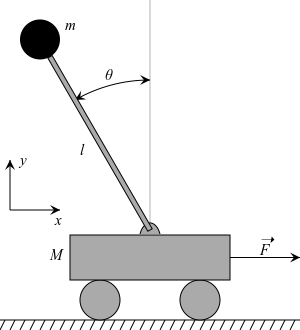
\includegraphics[width=7cm]{images/pendulum.png}
    \caption{The inverted pendulum model}
    \label{fig:pendulum}
\end{figure}

\emph{Consider a cart with an inverted pendulum hinged on top of it as shown in the Figure \ref{fig:pendulum}. For simplicity, the cart and the pendulum are assumed to move in only one plane, and the friction, the mass of the stick, and the gust of wind are disregarded. The problem is to maintain the pendulum at the vertical position. For example, if the inverted pendulum is falling in the direction shown, the cart moves to the right and exerts a force, through the hinge, to push the pendulum back to the vertical position.}\\
\emph{Let's consider the linearized inverted pendulum system (assuming $\theta(t)$ and $\Dot{\theta}(t)$ are very small)}

\begin{equation}
\begin{bmatrix}
    \Dot{x}_1(t) \\ \Dot{x}_3(t) \\ \Dot{x}_3(t) \\  \Dot{x}_4(t) \\ 
\end{bmatrix}
=
\begin{bmatrix}
    0 & 1 & 0 & 0 \\
    0 & 0 & -\frac{mg}{M} & 0 \\
    0 & 0 & 0 & 1 \\
    0 & 0 & \frac{(M+m)g}{Ml} & 0 
\end{bmatrix}
\begin{bmatrix}
    x_1(t) \\ x_2(t) \\ x_3(t) \\ x_4(t)
\end{bmatrix}
+
\begin{bmatrix}
    0 \\ \frac{1}{M} \\ 0 \\ - \frac{1}{Ml}
\end{bmatrix}
u(t)
\end{equation}
\emph{where $x_1(t) = x(t), \smallspace x_2(t) = \Dot{x}(t), \smallspace x_3(t) = \theta(t), \smallspace and \smallspace x_4(t) = \Dot{\theta}(t)$.}\\
\emph{Consider the LQR problem}

\begin{align}
    &u^* := \argmin_{u:[0,\infty) \to \mathbb{R}^m} J(u) := \int_0^\infty \left( x(t)^T Qx(t) + u(t)^T R u(t) \right) dt \\
    &\text{subject to}\\
    &\Dot{x}(t) = Ax(t) + Bu(t), \smallspace x(0) = x_0
\end{align}

\emph{where A and B are appropriate system matrices with m=1, M=2, l=3 and g=9.8.} \\
\emph{Tasks:}

\begin{enumerate}
    \item \emph{Appropriately choose the weighting $Q \geq 0$ and $R > 0$ to maintain the pendulum at the vertical position, i.e., $\theta(t) = 0$ and $\Dot{\theta}(t) = 0$ as much as possible.}
    \item \emph{Find an optimal policy for the LQR problem using Python or Matlab functions.}
    \item \emph{Plot trajectories of the system x(t) and the control input u(t) over certain time interval to demonstrate the performance of your optimal control policy.}
    \item \emph{In the answer, please include your Python or Matlab codes.}
    \item \emph{Change the weight and see how the performance changes and discuss about the results.}
\end{enumerate}
\\
\\
\textbf{Solution:}\\
\\

We want to keep the pendulum in the upright position as much as possible. Therefore, we can choose the values of $Q$ and $R$ as following:
\begin{itemize}
    \item Matrix $Q$: the values on the diagonal of the $Q$ matrix act as "penalties" for the corresponding state variable i.e. we want the $\theta, \dot{\theta}$ as small as possible hence they have a greater penalty. As such, the designed matrix is:
    \begin{equation}
        Q = \begin{bmatrix}
             1 & 0 & 0 &  0\\
             0 & 1 & 0 & 0\\
             0 & 0 & 100 & 0\\
             0 & 0 & 0 & 100\\
        \end{bmatrix}
    \end{equation}
    where the greater values correspond to the \emph{penalties} for $\theta$ and $\dot{\theta}$
    \item Matrix $R$: in this case we just have a uni-dimensional matrix. The larger the $R$ value, the larger the penalty on the input $u(t)$ and therefore the system will use less energy. We set
    \begin{equation}
        R = \begin{bmatrix}
            0.1\\
        \end{bmatrix}
    \end{equation}
\end{itemize}

The Python code for setting the matrices is as following:
\begin{minted}{python}
# Import libraries
import numpy as np
import torch
import scipy.linalg

# Parameters
m = 1 # pendulum mass
M = 2 # cart mass
l = 3 # pendulum length
g = 9.8 # gravity acceleration

# Build matrices
A = np.array([[0, 1, 0, 0], 
              [0, 0, -m*g/M, 0],
              [0, 0, 0, 1], 
              [0, 0, (M+m)*g/(M*l), 0]])
B = np.array([[0], [1/M], [0], [-1/(M*l)]])
rho = 0.1
Q = np.matrix([
    [1, 0, 0,   0],
    [0, 1, 0,   0],
    [0, 0, 100, 0],
    [0, 0, 0, 100]])
R = rho * np.eye(1) # control size is 1
\end{minted}

Then we define the LQR controller as following, where $X$ is the solution to the Riccati equations solved via the Python library \href{https://www.scipy.org/}{SciPy}. The closed loop gain $K$ is then defined as:
\begin{equation}
    K = R^{-1} B^T X
\end{equation}

Python code:
\begin{minted}{python}
def LQR(A,B,Q,R):
    """Solve the continuous time lqr controller.
    dx/dt = A x + B u
    cost = integral x.T*Q*x + u.T*R*u
    """
    #ref Bertsekas, p.151

    # First, try to solve the Riccati equation
    X = np.matrix(scipy.linalg.solve_continuous_are(A, B, Q, R))

    # Compute the LQR gain
    K = np.matrix(scipy.linalg.inv(R)*(B.T*X))

    eigVals, eigVecs = scipy.linalg.eig(A-B*K)

    return K, X, eigVals

K, X, eigVals = LQR(A, B, Q, R)

\end{minted}

By running the code with our designed controller we get:
\begin{equation}
    K = \begin{bmatrix}
        -3.16227766  & -9.26594071 &-146.94265769 & -80.13776765\\
    \end{bmatrix}
\end{equation}
In order to simulate the system, we design a class simulating the inverted pendulum and its physical behavior in time, which is discretized in steps of $\tau = 0.02s$:

\begin{minted}{python}
class ControlledPendulum():
''' Continuous version of the OpenAI Gym cartpole '''
def __init__(self, M, m, l, tau=0.02, g=9.81):
    self.gravity = g
    self.masscart = M
    self.masspole = m
    self.total_mass = (self.masspole + self.masscart)
    self.length = l  # actually half the pole's length
    self.polemass_length = (self.masspole * self.length)
    self.force_mag = 30.0
    self.tau = tau  # seconds between state updates
    self.state = None # Initialize through reset
    
def step(self, force):
    x, x_dot, theta, theta_dot = self.state
    costheta = math.cos(theta)
    sintheta = math.sin(theta)
    temp = (force + self.polemass_length * theta_dot \
        * theta_dot * sintheta)/ self.total_mass
    thetaacc = (self.gravity * sintheta - costheta * temp) / \
        (self.length * (4.0/3.0 - self.masspole * \
        costheta * costheta / self.total_mass))
    xacc = temp - self.polemass_length * thetaacc * \ 
        costheta / self.total_mass
    x = x + self.tau * x_dot
    x_dot = x_dot + self.tau * xacc
    theta = theta + self.tau * theta_dot
    theta_dot = theta_dot + self.tau * thetaacc
    self.state = x, x_dot, theta, theta_dot # save state
    return np.array(self.state, dtype='float64').reshape(4,1)

def reset(self, x_initial= [1, 0, 0, 0], random=False):
    # We can also simulate a disturbance from a random distribution
    if random == True:
        self.state = np.random.uniform(-0.1, 0.1, size=4)
    else:
        self.state = x_initial
    return np.array(self.state, dtype='float64').reshape(4,1)
\end{minted}

We can now start the simulation. We set up the model and set as initial state:
\begin{equation}
    x_0 = \begin{bmatrix}
        1\\
        0\\
        0\\
        0\\
    \end{bmatrix}
\end{equation}

The optimal control input is calculated at each time instant as 
\begin{equation}
    u^*(t) = -K x(t) 
\end{equation}
We simulate $10$ seconds with the following Python code:

\begin{minted}{python}
# Start from position -1 meter
x0 = [-1, 0, 0, 0] 

# Set the model to the initial position
x = model.reset(x_initial=x0, random=False)

# Save trajectory for the graph
trajectory = []
controls = []

# Control loop
for i in range(500):
    u = - K.dot(x)  # the control input is u* = -Kx
    x = model.step(u) # propagate
    trajectory.append(x)
    controls.append(u)
\end{minted}

\paragraph{Position and velocity plots}
We use the following code for plotting: 
\begin{minted}{python}
# Trajectory plotting
import matplotlib.pyplot as plt

tau = 0.02 # time of system update
tot_time = tau*len(trajectory)
t = np.linspace(0, tot_time, len(trajectory)) # time

x_traj, xdot_traj, theta_traj, thetadot_traj, 
    ctrl_traj = [], [], [], [], []
for i in range(len(trajectory)):
    x_traj.append(trajectory[i][0][0])
    xdot_traj.append(trajectory[i][1][0])
    theta_traj.append(trajectory[i][2][0])
    thetadot_traj.append(trajectory[i][3][0])
    ctrl_traj.append(controls[i][0][0].item())
    
fig, ax = plt.subplots(1,1, figsize=(16, 8))
ax.plot(t, x_traj, "k", alpha=.8, label=r'$x(t)$ [$m$]')
ax.plot(t, xdot_traj, "-.k", alpha=.8, label=r'$\dot{x}(t)$ [$m/s$]')
ax.plot([0, tot_time], [0, 0], ":b", alpha=.5, label=r'Setpoint')
ax.legend(loc='upper right')
ax.set_xlabel(r'Time [$s$]')
ax.set_ylabel(r'Value')
ax.set_title("Position and velocity plot")
fig.savefig('images/pendulum_pos_vel.jpg')
\end{minted}
We get the following result:
\begin{figure}[h!]
    \centering
    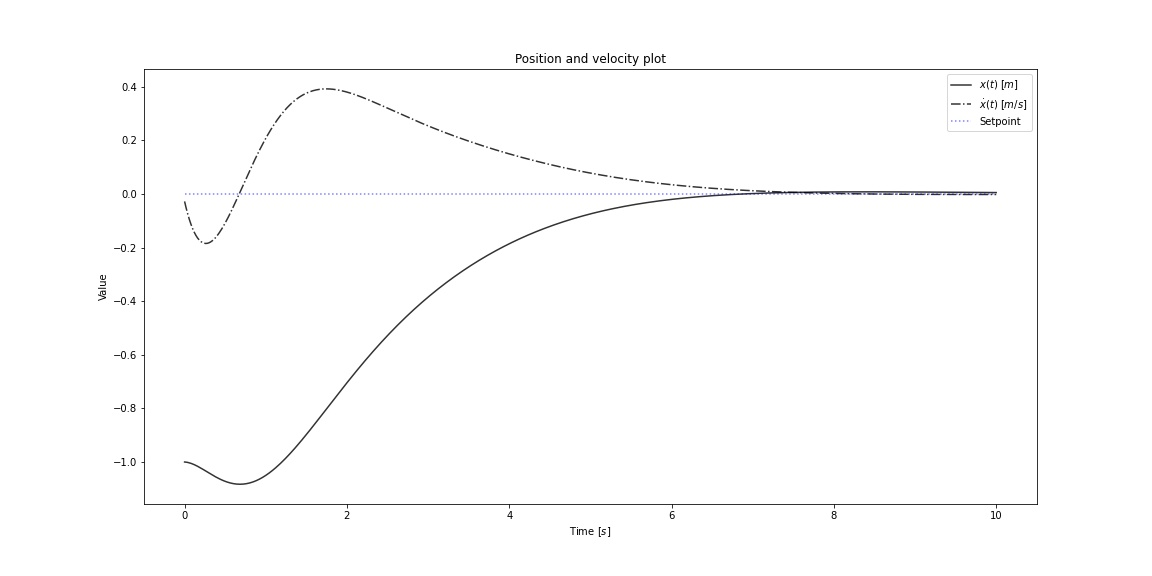
\includegraphics[width=\textwidth]{images/1-pendulum_pos_vel.jpg}
    \caption{Position and velocity plot}
    \label{fig:cartpole_posvel}
\end{figure}
We can see from Figure \ref{fig:cartpole_posvel} that the system is able to stabilize both the position and velocity of the system.

\paragraph{Angular position and angular velocity plots}
Using the following code we obtain
\begin{minted}{python}
fig, ax = plt.subplots(1,1, figsize=(16, 8))
ax.plot(t, theta_traj, "g", alpha=.8,label=r'$ \theta (t)$ [$rad$]')
ax.plot(t, thetadot_traj, "-.g", alpha=.8,label=r'$\dot{ \theta }(t)$ [$rad/s$]')
ax.plot([0, tot_time], [0, 0], ":b", alpha=.5, label=r'Setpoint')
ax.legend(loc='upper right')
ax.set_xlabel(r'Time [$s$]')
ax.set_ylabel(r'Value')
ax.set_title("Angular position and angular velocity plot")
fig.savefig('images/pendulum_angular_pos_vel.jpg')
\end{minted}

\begin{figure}[h!]
    \centering
    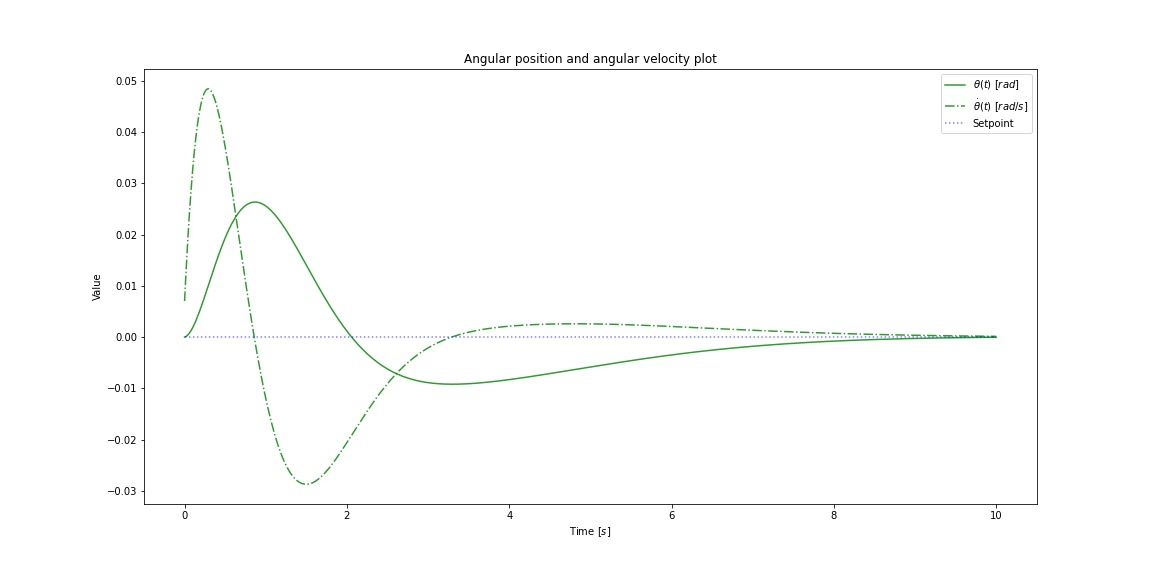
\includegraphics[width=\textwidth]{images/1-pendulum_angular_pos_vel.jpg}
    \caption{Angular positions and velocities}
    \label{fig:cartpole_ang}
\end{figure}

We can infer from Figure \ref{fig:cartpole_ang} that the system is able to stabilize both the angular position and angular velocity of the system and that their values are indeed very close to $0$.

\paragraph{Control input plots}
Using the following code we obtain
\begin{minted}{python}
fig, ax = plt.subplots(1,1, figsize=(16, 8))
ax.plot(t, ctrl_traj, "r", alpha=.6,label=r'$ u^*(t)$ [$N$]')
ax.plot([0, tot_time], [0, 0], ":b", alpha=.5, label=r'Setpoint')
ax.legend(loc='upper right')
ax.set_xlabel(r'Time [$s$]')
ax.set_ylabel(r'Value')
ax.set_title("Control input")
fig.savefig('images/pendulum_input.jpg')
\end{minted}

\begin{figure}[h!]
    \centering
    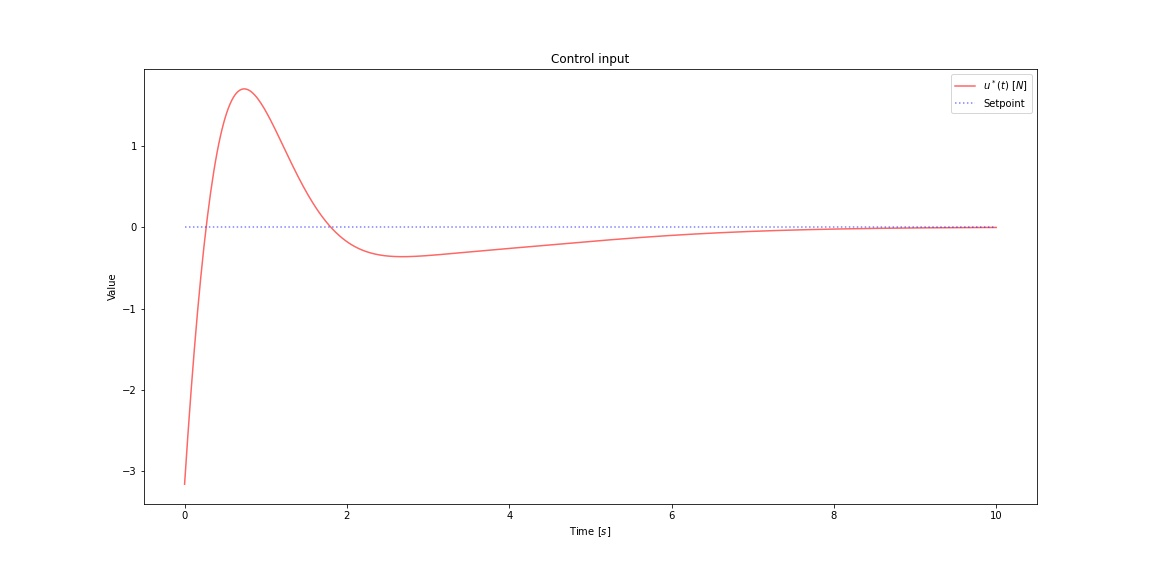
\includegraphics[width=\textwidth]{images/1-pendulum_input.jpg}
    \caption{Control input plot}
    \label{fig:cartpole_input}
\end{figure}

We can see from Figure \ref{fig:cartpole_input} that the system is using a control input $u(t)$ which is able to stabilize the state. Moreover, as expected, $\lim_{t \to \infty} u(t) = 0$.

\paragraph{Changing the weights}
We can now try to change the weights to see how the system performance changes. Let's say we want to penalize the position variation more in order to get a faster stabilization of the position and velocity. We design the matrix $Q$ as: 

\begin{equation}
    Q = \begin{bmatrix}
         100 & 0 & 0 &  0\\
         0 & 100 & 0 & 0\\
         0 & 0 & 100 & 0\\
         0 & 0 & 0 & 100\\
    \end{bmatrix}
\end{equation}

while keeping all the other parameters the same for a fair comparison. We get the control input gain as:
\begin{equation}
    K = \begin{bmatrix}
        -31.6227766  & -69.00397721 & -612.25803618  & -334.32523211\\
    \end{bmatrix}
\end{equation}
By comparison with the previous gain, we notice that the absolute value of the parameters is higher; this will result in a more "aggressive" control.
The plot are the following, in the same order as the experiment before in the below plots.
\begin{figure}[h!]
    \centering
    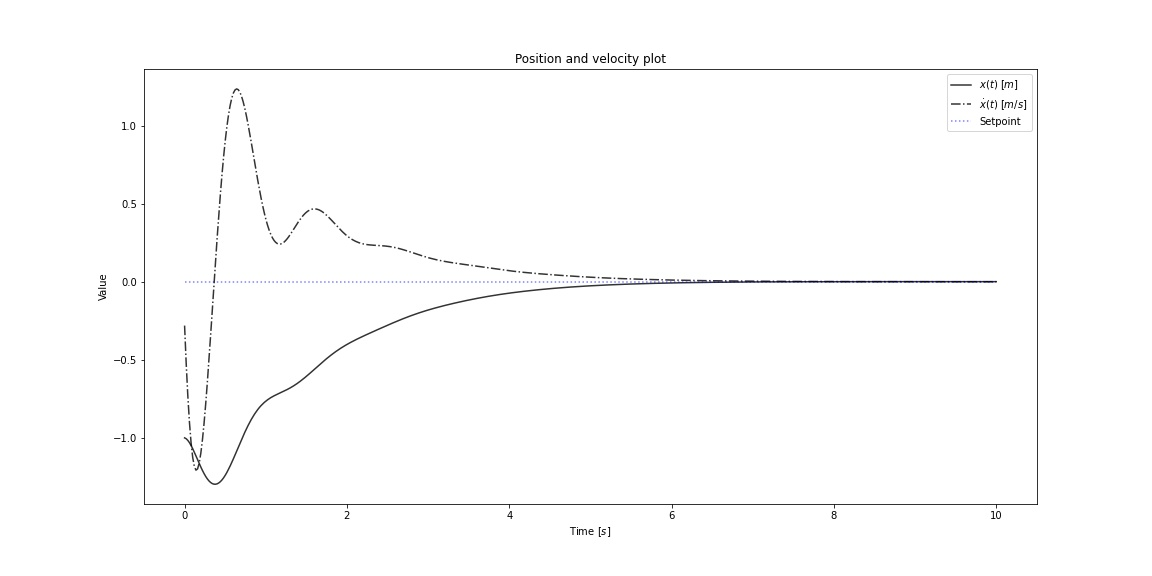
\includegraphics[width=\textwidth]{images/2-pendulum_pos_vel.jpg}
    \label{fig:pen_pos}
    \caption{New position and velocity plot}
\end{figure}
\begin{figure}[h!]
    \centering
    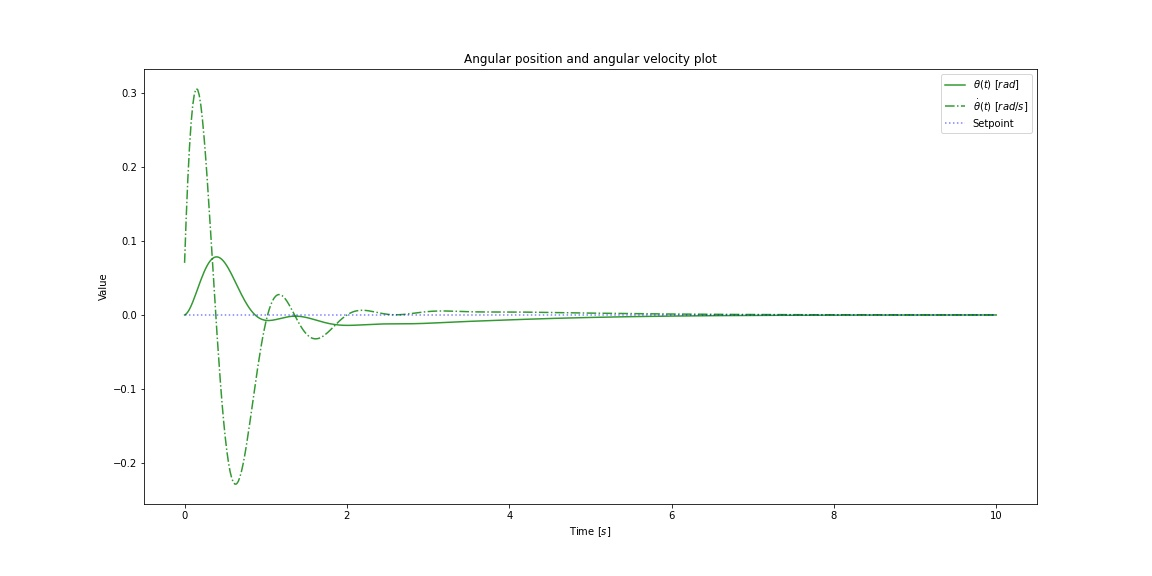
\includegraphics[width=\textwidth]{images/2-pendulum_angular_pos_vel.jpg}
    \label{fig:pen_an}
    \caption{New angular position and angular velocity plot}

\end{figure}
\begin{figure}[h!]
    \centering
    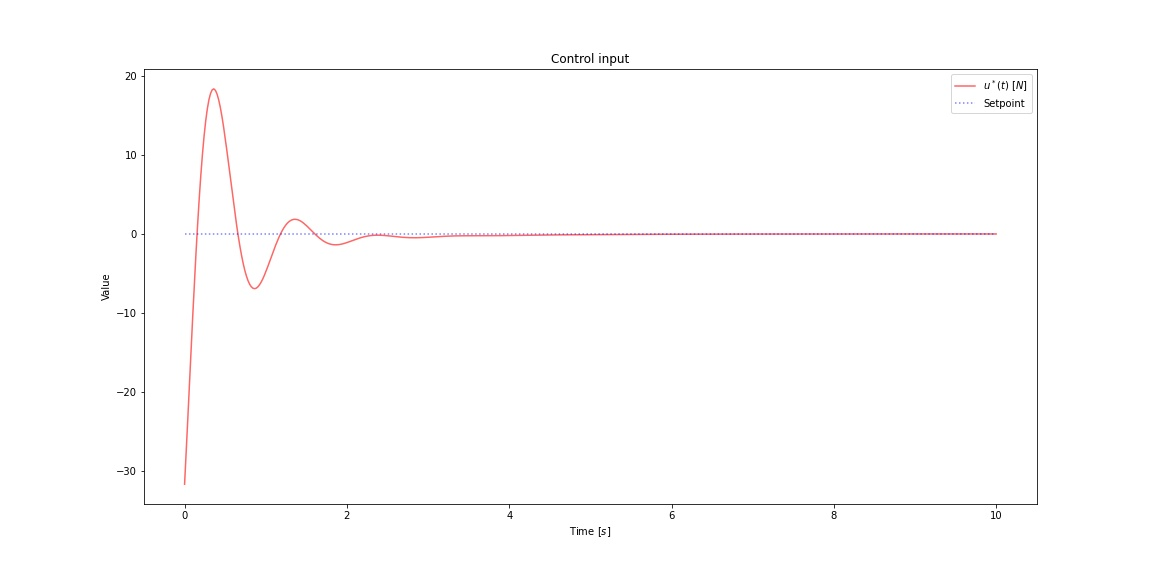
\includegraphics[width=\textwidth]{images/2-pendulum_input.jpg}
    \label{fig:pen_in}
    \caption{New control input plot}
\end{figure}

These results confirm our hypothesis: the position and velocity stabilize faster, at the cost of a higher variation for the angular position and velocity. Moreover, since the weight for the control input was chosen as $0.1$, its absolute value is much larger than before; the first was in the range of $u(t) \in (-4, 2)$ while the new control input has a much wider range around $u(t) \in (-40, 20)$. Thus, a more aggressive controller results in using more energy for a faster stabilization.
\section{Exercises from Lecture 6}

%%%%%%%%%%%%%%%%%%%%%%%%%%%%%%%%%%%%%%%%%%%%%%%%%%%%%%%%%%%%%%%%%%%%
\subsection{Exercise 6.15}
\emph{Consider the double integrator}
\begin{align}
    &\Dot{x}_1(t) = x_2(t), \\
    &\Dot{x}_2(t) = u(t)
\end{align}
\emph{and the cost}
\begin{equation}
    J(u) = \int_{t_0}^\infty \left( x_1(t)^2 + x_2(t)^2 + u(t) ^2 \right) dt
\end{equation}
\emph{Find P by solving the ARE. Verify (either analytically or numerically) that it is indeed the steady-state solution of the RDE.}
\\
\\
\textbf{Solution:}\\
\\
In order to solve the Algebraic Riccati Equation, we have to find the matrices defining the system. In this case, we have:
\begin{equation}
    A = \begin{bmatrix}
         0 & 1 \\
         0 & 0 \\
    \end{bmatrix}
    ,\smallspace B=
    \begin{bmatrix}
         0 \\
         1 \\
    \end{bmatrix}
    , \smallspace Q =
    \begin{bmatrix}
         1 & 0\\
         0 & 1\\
    \end{bmatrix}
    , \smallspace R =
    \begin{bmatrix}
         1 \\
    \end{bmatrix}
\end{equation}
We can now use the Python's library \href{https://www.scipy.org/}{SciPy} to solve the ARE:

\begin{minted}{python}
# Importing the packages
import numpy as np
from scipy.linalg import solve_continuous_are

# Build matrices
A = np.matrix([[0, 1],
               [0, 0]])
B = np.matrix([[0],[1]])
Q = np.eye(2) # Identity matrix, dim = 2
R = np.eye(1) # Identity matrix, dim = 1

# Solve the ARE
P = solve_continuous_are(A, B, Q, R)
print(P)
\end{minted}

By which we get 
\begin{equation}
    P = \begin{bmatrix}
         1.73205081 & 1 \\
         1 & 1.73205081 \\
    \end{bmatrix}
    \sim \begin{bmatrix}
         \sqrt{3} & 1 \\
         1 & \sqrt{3} \\
    \end{bmatrix}
\end{equation}

The formula for Riccati Differential Equation is as following:
\begin{equation}
    \Dot{P}(t) = -P(t)A - A^\top P(t) -Q + P(t) B R^{-1} B P(t) 
\end{equation}
So, based on the previous result we can get $ \Dot{P}(t) $ as following
\begin{minted}{python}
# Calculate the steady-state derivative
P_dot = A.T*P + P*A + Q -P*B*R*B.T*P 
print(P_dot)
\end{minted}
By which we get 
\begin{equation}
    \Dot{P} = \begin{bmatrix}
         0 & 0\\
         0 & 0\\
    \end{bmatrix}
\end{equation}
hence proving P is indeed the steady-state solution of the RDE.


%%%%%%%%%%%%%%%%%%%%%%%%%%%%%%%%%%%%%%%%%%%%%%%%%%%%%%%%%%%%%%%%%%%%
\subsection{Exercise 6.24}
\emph{Consider the infinite-horizon LQR problem}
\begin{align}
    &u^* := \argmin_{u:[0,\infty) \to \mathbb{R}} J(u) := \int_0^\infty \left( qx(t)^2 + ru(t)^2  \right) dt \\
    &\text{subject to}\\
    &\Dot{x}(t) = ax(t) + bu(t), \smallspace t \in [t_0, \infty) \\
    &x(t_0) = x_0
\end{align}

\emph{where $a, q, r > 0$ and $b \in \mathbb{R}$ is arbitrary. Find the optimal control law. Moreover, show that for $r \to 0 $,
the eigenvalue of the optimal closed-loop system moves off to $- \infty$, while for $r \to \infty$, the eigenvalue of the
optimal closed-loop system tends to $−a$}
\\
\\
\textbf{Solution:}\\
\\
Recalling the ARE as:
\begin{equation}
    0 = A^\top P + PA + Q -PBR^{-1}B^\top P
\end{equation}
the optimal control law will be given by:
\begin{align}
    &u^*(t) = K x^*(t)\\
    &\text{where the gain } K = -R ^{-1} B^\top P
\end{align}
with $P$ being the solution to the ARE. In this case, we have scalars instead of matrices, so the ARE becomes
\begin{align}
    &0 = aP + Pa +q - pb\frac{1}{r}bp\\
    &\Longrightarrow -\frac{b^2 P^2}{r} + 2aP + q = 0
\end{align}
Solving the equation, we get as a solution (choosing the positive sign, since we have the condition that $P \geq 0$):
\begin{equation}
    P = \frac{r \left(a  + \sqrt{a^2 + \frac{b^2 q}{r}} \right)}{b^2} 
\end{equation}

Therefore, the closed-loop gain $K$ becomes:
\begin{equation}
    K = - \frac{1}{r} b \frac{r \left(a +  \sqrt{a^2 + \frac{b^2 q}{r}} \right)}{b^{2}} = - \frac{a + \sqrt{a^2 + \frac{b^2 q}{r}}}{b}
\end{equation}
where $K \in \mathbb{R}$. The closed-loop system becomes:
\begin{equation}
    \Dot{x}^*(t) = Ax^*(t) + Bu^*(t) = (a - Kb)x^*(t)
\end{equation}
The eigenvalue of the closed loop system is the value of the scalar $a - Kb$ in this case.
\paragraph{Eigenvalues of the closed-loop system by changing $r$}
\begin{itemize}
    \item Case 1: $r \to 0$, we have the following limit for the gain $K$
    \begin{equation}
        \lim_{r \to 0} (a - Kb) = \lim_{r \to 0} a -  b \frac{a  + \sqrt{a^2 + \frac{b^2 q}{r}}}{b} = a - (a + \sqrt{a^2 +\infty}) = - \infty
    \end{equation}
    \item Case 2: $r \to \infty$, we have the following limit for the gain $K$
    \begin{align}
        \lim_{r \to \infty} (a - Kb) &= \lim_{r \to \infty} a -  b \frac{a  + \sqrt{a^2 + \frac{b^2 q}{r}}}{b} =\\ 
        &=a - (a + \sqrt{a^2 + \cancel{\frac{b^2 q}{\infty}}}) =  a - (a +\sqrt{a^2}) = -a 
    \end{align}
\end{itemize}

%%%%%%%%%%%%%%%%%%%%%%%%%%%%%%%%%%%%%%%%%%%%%%%%%%%%%%%%%%%%%%%%%%%%
\subsection{Exercise 6.25 (Boeing 747 Lateral Model)}
\emph{The complete lateral model of a Boeing 747 is}
\begin{align}
    &\Dot{x}(t) = Ax(t) + Bu(t) \\
    &y(t) = Cx(t) + Du(t)
\end{align}
\emph{where}
\begin{equation}
A = 
    \begin{bmatrix}
        -10 & 0 & 0 & 0 & 0 & 0 \\
        0.0729 & -0.0558 & -0.997 & 0.0802 & 0.0415 & 0 \\
        -4.75 & 0.598 & -0.115 & -0.0318 & 0 & 0 \\
        1.53 & -3.05 & 0.388 & -0.465 & 0 & 0 \\
        0 & 0 & 0.0805 & 1 & 0 & 0 \\
        0 & 0 & 1 & 0 & 0 & -0.3333 \\
    \end{bmatrix}
    , \smallspace B =
    \begin{bmatrix}
        1\\ 0\\ 0\\ 0\\ 0\\ 0\\
    \end{bmatrix}
\end{equation}
\emph{and}
\begin{equation}
    C =
    \begin{bmatrix}
        0 & 0 & 1 & 0 & 0 & -0.3333
    \end{bmatrix}
    , \smallspace D=0
\end{equation}

\emph{Minimize the sum of the energy of the output y and the energy of the control u. The main effort is to minimize the energy of y which is supposed to be zero in a steady state condition. So we put a weight $q = 9.527 > 1$ on the energy of y. The problem now is as follows.}

\begin{align}
    &u^* := \argmin_{u:[0,\infty) \to \mathbb{R}} J(u) := \int_0^\infty [qy(t)^Ty(t) + u(t)^2] dt \\
    &\text{subject to}\\
    &\Dot{x}(t) = Ax(t) + Bu(t), \smallspace t \in [t_0, \infty) \\
    &y(t) = Cx(t) + Du(t), \smallspace t \in [t_0, \infty) \\
    &x(t_0) = x_0
\end{align}
\emph{Tasks:}

\begin{enumerate}
    \item \emph{Find an optimal policy for the LQR problem by solving ARE using Python or Matlab functions.}
    \item \emph{Plot trajectories of $y(t)$ and $u(t)$.}
    \item \emph{In the answer, please include your Python or Matlab codes.}
\end{enumerate}
\\
\\
\textbf{Solution:}\\
\\
First of all, we need to find the matrix $Q$. We can see that, given $D = 0$, then
\begin{align}
    &y(t) = Cx(t)\\
    &\Longrightarrow J(u) := \int_0^\infty [x^T(t)(C^T q C ) x(t) + u(t)^2] dt
\end{align}
hence we can consider $Q = C^T q C$.
We solve the problem in Python. The first step is declaring all the variables:

\begin{minted}{python}
import numpy as np
import torch
import scipy.linalg

# Build matrices
A = np.matrix([[-10, 0, 0, 0, 0, 0],
              [0.0729, -0.0558, -0.997, 0.0802, 0.0415, 0],
              [-4.75, 0.598, -0.115, -0.0318, 0, 0],
              [1.53, -3.05, 0.388, -0.465, 0, 0],
              [0, 0, 0.0805, 1, 0, 0],
              [0, 0, 1, 0, 0, -0.3333]])
B = np.matrix([[1], [0], [0], [0], [0], [0]])
C = np.matrix([0, 0, 1, 0, 0, -0.3333])
D = 0*np.eye(1)

# Choose Q and R matrices
q = 9.527
Q = C.T*q*C
R = np.eye(1)
\end{minted}


Then we define the LQR controller as following, where $X$ is the solution to the Riccati equations solved via the Python library \href{https://www.scipy.org/}{SciPy}. The closed loop gain $K$ is then defined as:
\begin{equation}
    K = R^{-1} B^T X
\end{equation}

Python code:
\begin{minted}{python}
def LQR(A,B,Q,R):
    """Solve the continuous time lqr controller.
    dx/dt = A x + B u
    cost = integral x.T*Q*x + u.T*R*u
    """
    #ref Bertsekas, p.151

    # First, try to solve the Riccati equation
    X = np.matrix(scipy.linalg.solve_continuous_are(A, B, Q, R))

    # Compute the LQR gain
    K = np.matrix(scipy.linalg.inv(R)*(B.T*X))

    eigVals, eigVecs = scipy.linalg.eig(A-B*K)

    return K, X, eigVals

K, X, eigVals = LQR(A, B, Q, R)

\end{minted}

By running the code with our designed controller we get the gain as
\begin{equation}
    \begin{bmatrix}
         1.05951967 &-0.19104882 &-2.31972318 & 0.09916995 & 0.03704914 & 0.48581648\\
    \end{bmatrix}
\end{equation}

In order to simulate the system, we design a class simulating the lateral model of the Boeing 747 and its physical behavior in time, which is discretized in steps of $\tau = 0.02s$:

\begin{minted}{python}
class ControlledBoeing747():
    def __init__(self, A, B, C, D, dt = 0.02):
        """ Simulate the system by calculating the state 
        variation with: x_{t+1} = x_t + dx*dt
        where dx = Ax + Bu and y = Cx +Du
        
        The variables are:
        dt: time step (i.e. 0.02s) to forward propagate the simulation
        x: current state
        A, B, C, D: matrices describing the dynamics
        """
        self.dt = dt # Time step, i.e. 0.02s
        self.A = A
        self.B = B
        self.C = C
        self.D = D
    
    # Simulate next step
    def step(self, u):
        dx = A*self.x + B*u
        self.x += dx*self.dt # x_{t+1} = x_t + dx*dt
        output = C*self.x + D*u
        return self.x, output
    
    # Reset to initial position
    def reset(self, x_initial= 
              np.matrix(np.random.uniform(-0.1, 0.1, size=6)).T):
        self.x = x_initial
        return self.x
\end{minted}
 
 We set as initial condition the following $x_0$ with the Numpy's random function generator: 
 \begin{minted}{python}
# Declare model
model = ControlledBoeing747(A, B, C, D)

# Initial condition
x0 = np.matrix(np.random.uniform(-0.5, 0.5, size=6)).T    
model.reset(x_initial=x0)
 \end{minted}
and then we run for $1000$ time steps, equivalent to a simulation of $20$ seconds:
\begin{minted}{python}
# Save trajectory for the graph
trajectory_state = []
trajectory_outputs = []
controls = []

# Control loop (each loop is 0.02s of simulation)
for i in range(1000):
    u = - K*x  # the control input is u* = -Kx
    x, y = model.step(u) # propagate
    trajectory_state.append(x)
    trajectory_outputs.append(y)
    controls.append(u)
\end{minted}
 
\paragraph{Output plot} We use the following functions to get the plot:

\begin{minted}{python}
# Trajectory plotting
import matplotlib.pyplot as plt

tau = 0.02 # time of system update
tot_time = tau*len(trajectory_outputs)
t = np.linspace(0, tot_time, len(trajectory_outputs)) # time

y, u = [], []
for i in range(len(trajectory_outputs)):
    y.append(trajectory_outputs[i].item())
    u.append(controls[i].item())

fig, ax = plt.subplots(1,1, figsize=(16, 8))
ax.plot(t, y, "k", alpha=.8, label=r'$y(t)$')
ax.plot([0, tot_time], [0, 0], ":b", alpha=.5, label=r'Setpoint')
ax.legend(loc='upper right')
ax.set_xlabel(r'Time [$s$]')
ax.set_ylabel(r'Value')
ax.set_title("Output $y(t)$ plot")
fig.savefig('images/boeing_output.jpg')
  
\end{minted}

\begin{figure}[h!]
    \centering
    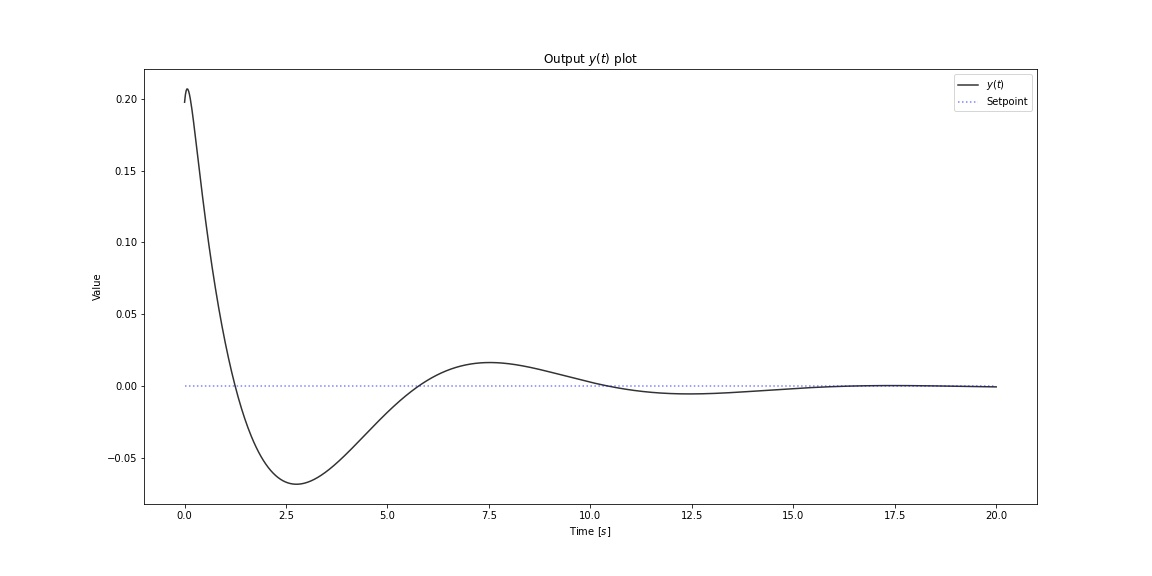
\includegraphics[width=\linewidth]{images/boeing_output.jpg}
\end{figure}

\paragraph{Control input plot} We use the following code for plotting the control input:

\begin{minted}{python}
fig, ax = plt.subplots(1,1, figsize=(16, 8))
ax.plot(t, u, "r", alpha=.8,label=r'$u(t)$')
ax.plot([0, tot_time], [0, 0], ":b", alpha=.5, label=r'Setpoint')
ax.legend(loc='upper right')
ax.set_xlabel(r'Time [$s$]')
ax.set_ylabel(r'Value')
ax.set_title(r"Control input $u(t)$ plot")
fig.savefig('images/boeing_input.jpg')
\end{minted}

\begin{figure}[h!]
    \centering
    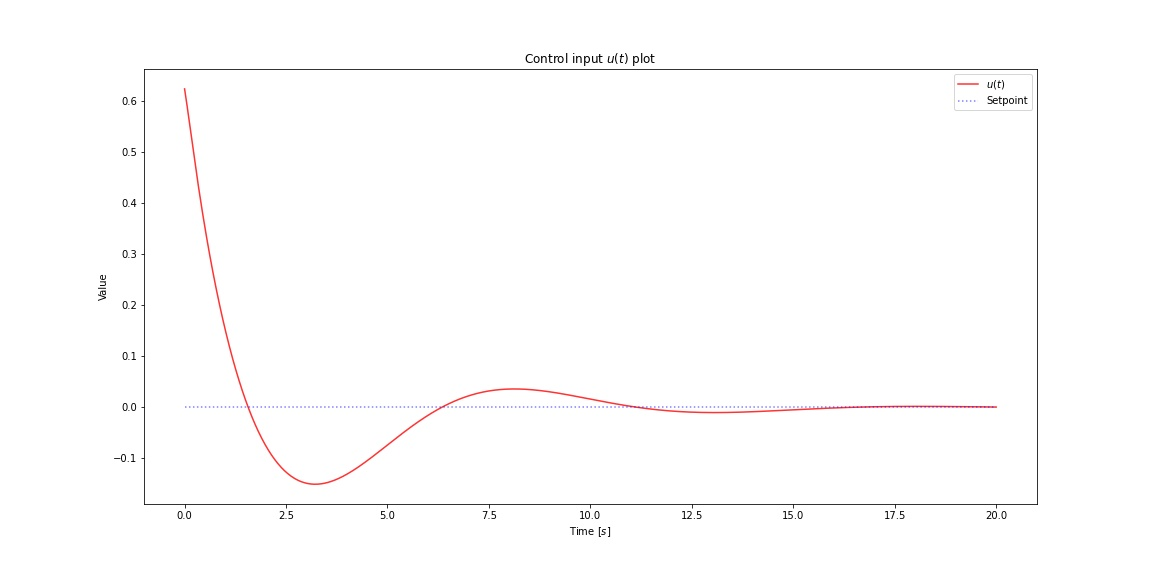
\includegraphics[width=\linewidth]{images/boeing_input.jpg}
\end{figure}

As we can see from the graphs, the LQR controller is able to stabilize the output and bring it to a stable state within the time span we set. Moreover, as we expected, the control input satisfies the condition that $\lim_{t \to \infty} u^*(t) = 0$ and also zeroes out the output in the steady state.

\end{document}